\chapter{Entrenamiento de modelos completos sobre la base de datos}

Tras las descripción de los modelos a utilizar, y las funciones de pérdida a emplear, comienza el proceso de entrenamiento de los modelos. Este proceso es uno de los más lentos de todo el desarrollo del proyecto, debido a la cantidad de horas necesarias a esperar para recopilar los resultados del modelo. Se estudiará la eficiacia de cada modelo a la hora de evaluar el problema, y las decisiones tomadas para su mejora y elección.\\

Para resolver este problema, se ha tomado un enfoque de dos niveles; en primer lugar, distinguiremos si la enfermedad que se recibe como entrada se trata de un ejemplar de enfermedad maligna o benigna, y posteriormente, su salida indicará un segundo modelo a aplicar sobre la enfermedad, especializado únicamente en uno de los dos tipos de enfermedades. Así, conseguimos un conjunto de modelos especialziados que permiten otorgar el diagnóstico con mayor precisión y seguridad.\\

Un aspecto clave de este proceso será la eficiencia, pero sobre todo el correcto diagnóstico de las enfermedades, por lo que usaremos como métricas de selección precision, el recall y balanced accuracy:

\begin{itemize}
	\item Precision. Proporción de valores bien clasificados dentro de una clase teniendo en cuenta verdaderos y falsos positivos. $$Precision=TP / (TP + FP).$$
	\item Recall. Valores correctamente identificados como positivos respecto al total de elementos positivos. $$Recall = TP / P$$
	\item Balanced accuracy: combina sensitivity y specificity. La primera, devuelve el valor real de proporción de valores correctamente clasificados entre el total de casos positivos que tenemos (contando predicciones positivas y falsos negativos), mientras que la especifidad, nide el caso dual: la proporción de casos negativos bien clasificados respecto al total de datos negativos tanto bien clasificados como mal clasificados, y que son identificados como falsos positivos. Esto nos permite calcular el accuracy de forma proporcional al porcentaje de presencia de las clases, e intentamos así paliar el efecto del desequilibrio de los datos:
	$$Sensitivity = TP/(TP+FN)$$
	$$Specificity =(TN/(TN+FP)$$\\
$$ Balanced\ accuracy: \frac{Sensitivity + Specificity}{2}$$
	
	En base a esta expresión, podemos saber que si el valor es aproximadamente 1/númeroClases, es posible que gran parte de las clases no estén siendo correctamente clasificadas en caso de ser minoritarias. Valores mayores nos harán conocer que el resultado de clasificar todas las clases es satisfactorio.
\end{itemize}

\section{Clasificación binaria}

El problema de la clasificación binaria consiste en la distinción de las enfermedades malignas de aquellas que son benignas. Se trata del primer problema a resolver antes de especificar el tipo de enfermedad que posee el paciente, y así poder especializar los modelos segundo nivel.

\subsection{Equilibrio de los datos}

El primer inconveniente que nos encontramos para este problema es el inmenso desbalaceo entre la clase benigna y maligna. Si redibujamos el gráfico mostrado durante la fase de preprocesamiento de datos, únicamente con los datos de entrenamiento, obtenemos lo siguiente: 

\begin{figure}[H]
	\centering
	\label {desequilibriototal}
	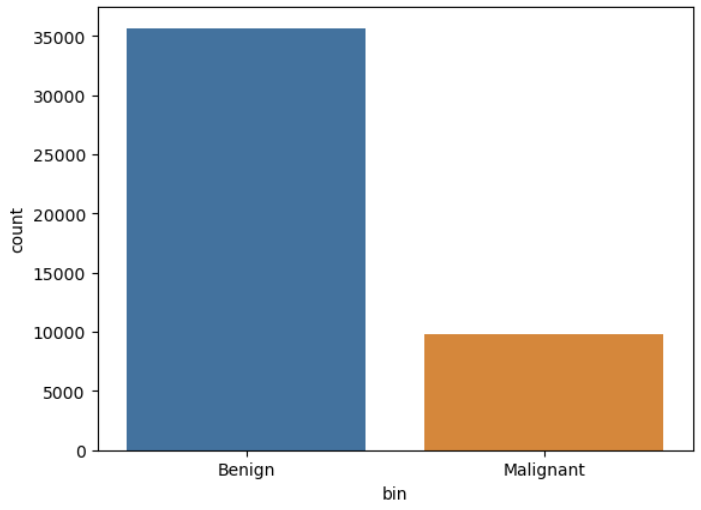
\includegraphics[scale = 0.4]{imagenes/desequilibriototal.png}
	\caption{Desequilibrio de datos}
\end{figure}

Se puede observar la alta disparidad existente entre ambas, siendo 35664 casos benignos y 9752 malignos. Es una diferencia de 3.65 veces más casos benignos que malignos, lo que se traduce en un equilibrio de  79\% y 21\% respectivamente. Para paliarlo, podemos efectuar dos estrategias: aplicar técnicas de oversampling (también conocido como sobremuestreo sintético), donwsampling de la clase mayoritaria, o bien, la aplicación de penalziaciones sobre la clase minoritaria para que su incorrecta clasificación tenga mayores consecuencias (haciendo uso de FocalLoss).\\

\subsubsection{Técnicas descartadas}

La ténica de downsampling de la clase mayoritaria queda descartada, debido a que dentro de esa clase, podemos encontrar etiquetas de segundo nivel asociadas a las enfermedades que se pueden diagnosticar. Como algunas de estas clases son muy escasas en número, si realizamos downsampling de forma aleatoria sin ningún tipo de restriccióin, podría darse el caso límite en la que una clase completa desapareciese del cojunto. Y esto conllevaría a la obtención de errores al evaluación de test, pues tendríamos una clase presente en test no estudiada en entrenamiento, que sólo provocaría un aumento de las métricas de error. \\

El uso de la función de pérdida FocalLoss podría ayudar a paliar este efecto. Sin embargo, debido al desajuste 79-21 del que disponemos, y la gran variedad de imágenes, se trata de una solución demasiado arriesgada. Para comprobarlo, se sometíó a evaluación con los valores por defecto recomendados de Resnet50. A priori, los resultados podrían parecer correctos en validación \ref{tab:resultsfl}; sin embargo, observamos que la clase minoritaria, la maligna, obtiene resultados que no están a la altura de la clase mayoritaria. Observamos un valor 0.41 en recall, valor preocupante frente al 0.95 de la clase benigna. Al existir un recall bajo, quiere decir que esta clase no se está detectando adecuadamente como maligna, y casi el 60\% de sus casos son calificados como benignos. Esto es un grave problema, ya que los casos malignos son los que más riesgo conllevan para la salud. Por tanto, se descarta también esta estrategia.


\begin{table}[!ht]
	\centering
	\begin{tabular}{|l|c|c|c|c|}
		\hline
		& Precision & Recall & F1-score & Support \\
		\hline
		Benign & 0.86 & 0.95 & 0.90 & 15338 \\
		Malignant & 0.68 & 0.41 & 0.51 & 4126 \\
		\hline
		Accuracy &  &  & 0.83 & 19464 \\
		Macro avg & 0.77& 0.68& 0.71&19464\\
		Weighted avg&0.82&0.83&0.82&19464\\
		\hline
	\end{tabular}
	\caption{Informe de clasificación}
	\label{tab:resultsfl}
\end{table}

\subsubsection{Propuesta: oversampling}

Sólo nos queda disponible la estategia de oversampling: la ampliación sintética de la clase minoritaria. Este proceso es muy delicado, ya que se basa en realizar alteraciones sobre las imágenes disponibles para dotarlas al conjunto de una mayor variabilidad, hasta equiparar el número de ejemplares con el de la clase mayoritaria. Existen distintas técnicas a aplicar, pero en este caso, utilizaré la estrategia de realizar alteraciones sobre las imágenes mediante una biblioteca de transformaciones: imgaug.

Se aplicarán una serie de transformaciones la imagen que alteren su estructura, pero con cuidado de no generar imágenes demasiado modificadas que se alejen de la distribución original de la clase maligna. Para realizar las transformaciones, he contruido un pipeline, una secuencia de transformaciones que aplica, en orden aleatorio, y con cierta probabilidad, las siguientes variaciones:

\begin{itemize}
	\item Fliplr(p=0.5). Se trata de un efecto de espejo de la imagen, respecto a su eje horizontal. Es equivalente a realizar una rotación de la imagen de 180º sobre su eje teórico horizontal que transcurre por la mitad de la imagen. Esta alteración se realziará con un 50\% de probabilidad.
	\item Flipud(p=0.5). Se trata de un efecto de espejo de la imagen, respecto a su eje vertical. Es un caso de efectos similares al anterior, aplicado con un 50\% de probabilidad.
	\item Gaussian blur (p=0.5). Se aplicará filtro gaussiano en el 50\% de los casos, especificándose un valor de sigma muy pequeño de 0.5.
	\item Modificación de contraste  (p=0.25). Se aplicará un aumento o decremento del contraste del 20\% en el 25\% de los casos. Esto emula posibles cambios de luminosidad ambiente y de profundidad de color de la cámara
	\item Ruido Gaussiano aditivo  (p=0.5). Se aplica en caso de que el ruido gaussiano estándar no sea aplicado. Aplica un filtro gaussiano a nivel de canal, de forma que solo parte de la imagen se encuentra difuminada.  Se aplica también en un 50\% de los casos
	\item Transformaciones afines  (p=0.2): se trata de una alteración compuesta de escala y zoom, y una posterior traslación o rotación de la imagen. Se trata de una opcionalidad ofrecida por imgaug de forma no configurable directamente.
\end{itemize}

Estos valores han sido escogidos tomando como inspiración las transformaciones realizadas por el equipo ganador de la competición de ISIC \cite{1stISIC}, debido a sus buenos resultados.

Es importante destacar que dichas transformaciones únicamente se han realizado sobre los datos de entrenamiento; los datos de validación y test permanecen inalterados de forma que éstos sigan siendo un estimador no sesgado del rendimiento del modelo. Poir tanto, la extracción del 30\% de validación se realiza antes del sobremuestreom y los dos subconjuntos se guardan en carpetas distintas, a las que llamaremos train y test.

\subsection{Representación en Pytorch}

Con los datos preparados, configurar mediante Fastai y Pytorch los modelos que deseamos probar. Los 3 modelos siguen la misma configuración, a excepción de la importación del modelo, por lo  que será explicado de forma paramétrica. Tenemos 3 tareas diferenciables: la creación del datablock para la gestión de los datos, el entrenamiento del modelo, y la transformación del mismo al modelo cuantizado empleado en el dispositivo Android.

\subsubsection{Creación del datablock}

FastAI ofrece el tipo de objeto Datablock para la creación de una estructura que organiza los datos de entrenamiento. Permite construir un bloque con todos los datos, de forma que cualquier consulta o verificación pueda realizarse sobre un mismo objeto. Consta de varios parámetros que podemos ajustar para normalizar las imágenes, adaptar el tamaño de entrada, o realizar la separación train-validación. Desglosadando los parámetros más importantes, tenemos:

\begin{itemize}
	\item blocks. Nos permite establecer el formato de entrada de datos, y la salida que queremos obtener de los mismos. En problemas de clasificación, habitualmente, tendremos como entrada un bloque de imágenes, y como salida, queremos obtener un conjunto de categorías asociados al bloque.
	\item get\_items. Establece la fuente de la cual obtener los datos para la construcción del DataBlock. Se trata de una función preconfigurada para la lectura de datos dado un repositorio o dirección de disco. En nuestro caso, como las imágenes no contienen información compleja, como plantillas de segmentación, se importan directamente de esta forma.
	\item splitter. Permite especificar divisiones de los datos. Habitualmente, se utiliza la función RandomSplitter, que nos permite separar los datos en entrenamiento y validación. Como parámetros de entrada, recibe el porcentaje de datos para validación que queremos obtener, y opcionalmente una semilla, por si deseamos repetibilidad de los experimentos. Como en este caso, queremos que el conjunto de entrenamiento sea el conjunto sobremuestreado, y validación, sea la carpeta valid, se ha creado una función que indica 1 si la imagen pertenece a la carpeta valid, y 0, si se encuentra en train. \ref{fig:particiones}
	\item get\_y. Parámetro al cual se asocian las etiquetas de los elementos de entrada. Puede recibir una función o bien una lista con las etiquetas asociadas a los elementos del dataset. FastAI toma las etiquetas por defecto del nombre de carpeta, por lo que tendremos que especificarle una función que tome la etiqueta del dataset \ref{fig:etiquetadobinario}.
	\item item\_tfms. Establece modificaciones sobre las imágenes de forma previa a la ejecución del modelo. En este caso, como ya hemos realizado oversampling, no realizaremos ninguna otra modificación sobre las imágenes para no transformar en exceso los datos.
	\item batch\_tfms. Permite realizar transformaciones a nivel de batch. Permite aplicar operaciones como la normalización de las imágenes. Este procedimiento favorece la convergencia del modelo, aunque el cálculo de la media y desviación típica es costoso. En su lugar, utilizaré la normalización que provee ImageNet, donde ya se incluyen los valores estadísticos de media y desviación para los datos en la variable *image\_stats provenientes de decenas de millones de imágenes.
	
\end{itemize}


 \begin{algorithm}[H]
	\caption{Función para la distinción de entrenamiento y validación}
	\label{fig:particiones}
	\begin{algorithmic}[1]
		
		\Procedure{ val\_splitter}{fname}
		\Comment{Comprueba si la carpeta contenedora es validiación}
		\State var pertenece: boolean = False
		\If{Path(fname).parent.name = valid}
			\State pertenece = True
		\EndIf \\
		\Return pertenece
		\EndProcedure
		
	\end{algorithmic}
\end{algorithm}

\begin{algorithm}[H]
	\caption{Función para la consulta de etiquetas}
	\label{fig:etiquetadobinario}
	\begin{algorithmic}[1]
		
		\Procedure{ binary\_label}{fname, df\_data: Dataframe}
		\State coincidence = $df\_data[i]$ where $df\_data[i] = fname, i \in Integer$
		\State var label = coincidence.label\\
		\Return label
		\EndProcedure
		
	\end{algorithmic}
\end{algorithm}

Una vez definido, podremos instanciar el datablock, configurando uno de los parámetros más críticos del entrenamiento: el tamaño de batch.

Cuando entrenamos una red, estamos ajustando una serie de pesos según recorremos los datos. Éstos, por tanto, pueden actualizarse en diferentes momentos: tras procesar cada imagen, tras procesarlas todas, y antes de volver a empezar, o cada n imágenes. A dicho tamaño n, se le conoce como tamaño de batch: es el tamaño del conjunto de imágenes que han de procesarse para realizar una actualización de pesos del modelo. 

Este número es un hiperparámetro clave, ya que tiene relación directa con la convergencia: a mayor tamaño, mayor velocidad de convergencia, pero menor precisión; y el caso inverso ocurre con el caso extremo, si, por ejemplo, actualizamos con cada ejemplar procesado. En la literatura, existen gran cantidad de estudios acerca de este valor, y establecen el valor adecuado en un intervalo $[2, 32]$,  compuesto únicamente por las potencias de 2   \cite{masters2018revisiting}. Debido a limitaciones de memoria, y la demostración de su optimalidad, emplearé tamaño 32 para los 3 modelos, aunque otros tamaños, como 64 o 128, también son viables.

A partir de ahora, denominaremos época al proceso de recorrer cada uno de los batches del datablock.

\subsubsection{Definición del modelo. Transfer learning}

Con los datos correctamente definidos, podemos construir el modelo propiamente dicho para el entrenamiento. En Fastai, la construcción de modelos puede hacerse de forma modular, mediante la especificación de las capas que componen la red, ya que la librería dispone de los módulos ya configurados a excepción de los canales de entrada y salida. A pesar de ello, la creación de un modelo desde cero es muy costoso computacionalmente, ya que se parte el entrenamiento de valores aleatorios. Por este motivo, normalmente se tiende a emplear modelos preentrenados, y adaptar su salida mediante el uso de transfer learning.

El transfer-learning es una métodología que permite utilizar complejas redes convolucionadas preeentrenadas con datasets de gran tamaño que son adaptadas para utilizarse con otros datasets diferentes y obtener buenos resultados, sin necesidad de realizar un entrenamiento desde cero del modelo.\\

De forma intuitiva, el proceso a seguir es el siguiente: partimos de las capas ocultas ya entrenadas del modelo, y sustituimos su cabecera por una nueva que se adapte a nuestro problema. Por cabecera(head), entendemos la parte final de la red, punto en el cual se elabora la salida final que la red pasa a la función SoftMax para obtener las probabilidades de pertenencia a cada clase de la imagen de entrada. Como la red fue entrenada para otro dataset, es probable que el número de clases de salidas sea diferente, y por eso, debemos de sustituirla por una nueva que se adapte a las necesidades de nuestro problema.\\

Una vez sustituida el head de la red, debemos de entrenar la nueva cabecera para que sus pesos se adapten a los datos de entrada y ofrezcan buenas métricas. Pero no nos interesa modificar el resto de capas ocultas, ya que fueron entrenadas previamente y tienen valores de W adecuados. Realizaremos un "congelado" de estas capas, para únicamente entrenar la nueva adición.

Posteriormente, para afinar el comportamiento de la red completa, ``descongelaremos'' la red para hacer un entrenamiento breve a la red completa, durante un número pequeño de épocas. Así, obtemos un modelo final adaptado a nuestro problema.\\

En esta primera fase, debemos ofrecer una salida binaria, que nos ofrezca una respuesta de 0 (benigno) y 1 (maligno). Para conseguirlo, recurriremos a retirar la capa predefinida con la que viene nuestro modelo, y para todos ellos, emplearemos la misma cabecera, la cual es creada de forma automática por fastai tras especificar el número de salidas.

\begin{table}[H]
	\centering
	\begin{tabular}{|c|c|c|}
		\hline
		\textbf{Capa} & \textbf{Tam. Entrada} & \textbf{Tam. Salida} \\ \hline
		Average pooling & n x n & 32 x 2048 \\ \hline
		Flatten & 32 x 2048 & 4096 \\ \hline
		Fully connected & 4096 & 512 \\ \hline
		Fully connected & 512 & 32 x 2048 \\ \hline
		Fully connected & 32 & 2 \\ \hline
		Softmax & - & - \\ \hline
	\end{tabular}
		\caption{Cabecera para trasfer-learning binario}
	\label{header}
\end{table}

Dicha cabecera, observable en la figura \ref{header}, recibe como tamaño de entrada n x n, siendo n el tamaño de la salida de la última capa de la red preentrenada que estemos utilizado. Mediante una oporación de average pooling, podemos convertir dicha entrada a un tamaño de salida concreto, el cual nos permitirá tener a partir de este punto una red totalmente conectada la cual no requiere ser modificada aunque modifiquemos el tamaño de entrada de la red por imágenes de mayor o menor resolución. \\

La configuración escogida tras el flattening de la imagen, que consiste en vectorizar su contenido, es una tradicional triple capa de redes totalmente conectadas: la estructura tradicional de una red neuronal donde cada neurona se encuentra conectada a las siguientes. Dicha estructura de entradas y salida sigue forma de ``embudo'', en el que el tamaño de la capa final coincide con el  número de salidas, en este caso, dos clases.

Para instanciar el modelo ya configurado, se hace uso de la clase vision\_learner, la cual recibe como entreada el modelo, expresado como cadena, un vector con los nombres de las métricas, el datablock de entrenamiento y validación creado anteriormente, y las funciones de callback. Estas últimas son funciones que serán ejecutadas cada vez que se complete una época de nuestro modelo. Como entrada, he decidido añadir un callback de salvado, que guarde el modelo tras cada época finalizada, y un monitor de Early stoping.


\begin{figure}[H]
	\centering
	\label {earlystopping}
	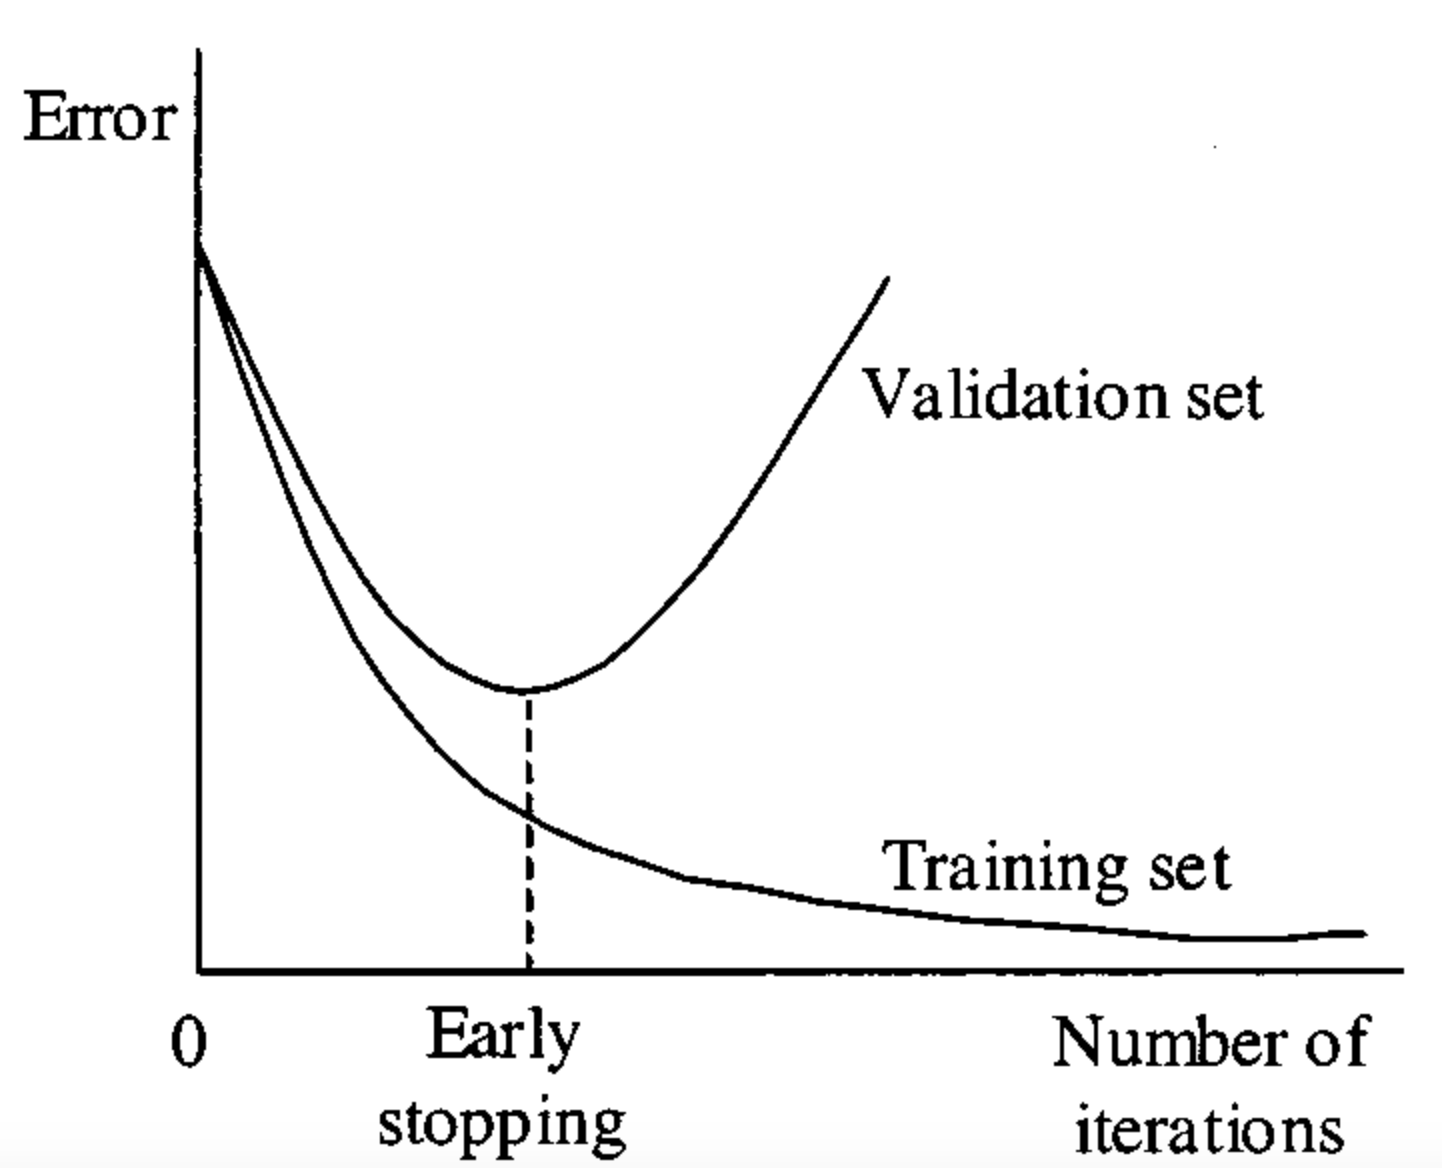
\includegraphics[scale = 0.17]{imagenes/earlystopping.png}
	\caption{Demostración gráfica del Early stopping \cite{earlystop}}
\end{figure}

Resumiendo, early stopping es un mecanismo de parada automática del entrenamiento, el cual, especificando una paciencia, en época, si no se cumple una condición, se detiene el modelo; en este problema, he decidido que el monitor de parada supervise el error de pérdida en validación, para así evitar el sobreaprendizaje de la red: la memorización completa del conjunto de entrenamiento, conllevando el riesgo de pérdida de generalidad. Controlaremos este fenómeno gráficamente mediante la muestra de las pérdidas de entrenamiento y validación.

\subsubsection{Entrenamiento}

El entrenamiento es la otra parte clave de la creación de modelos de deep learning. Esto se debe a la existencia de usa serie de hiperparámetros que debemos regular para asegurar el correcto entrenamiento del modelo. En este apartado, trataramos los dos parámetros clave: el número de épocas de entrenamiento, y el learning rate.

El número de épocas es equivalente al número de iteraciones realizadas sobre la totalidad de los datos del modelo, Éste debe ser fijado de forma estratégica para evitar que se produzca sobreentrenamiento, donde en lugar de aprender las características generales de los datos y su distribución, pasamos a su memorización completa. Este fenómeno, como ya se ha explicado, provoca pérdida de generalidad del modelo fuera del conjunto de entrenamiento, y no es lo deseable. En lugar de establecer dicho número de forma fija, usaremos, como ya enunciamos, Early stoping. De esta forma, será el propio modelo quien se detenga sin necesidad de que establezcamos un valor manual. Concretamente, emplearemos una paciencia de 3 épocas sobre la pérdida de validación.\\

En cuanto al learning rate, éste es un valor crítico para definir el tamaño de salto que se produce a la hora de optimizar el modelo. Define el tamaño del salto (step) que se produce a través del hiperplano definido por la función que modela los datos, en búsqueda de su mínimo local (o global). AL igual que el tamaño de batch, define de manera implícita la precisión de la búsqueda del óptimo; a mayor valor, mayor velocidad de convergencia, pero menor certeza de encontrar el óptimo de forma precisa; y a menor valor, mayor tiempo de entrenamiento, pero mayores garantías de encontrar un valor cercano al óptimo de la función.

La decisión de este parámetro normalmente se realiza mediante pruebas experimentales. Sin embargo, al disponer de recursos hardware limitados, no es posible realizar experimentos en paralelo en búsqueda de este valor, cuyo entrenamiento podría conllevar semanas. Por tanto, en lugar de usar un learning rate fijo, se ha tomado la decisión de usar un learning rate adaptativos, mediante la política de entrenamiento de un solo ciclo (Fit one cycle en FastAI) propuesta por Leslie Smith \cite{smith2018disciplined}.

Con esta técnica, el valor del learning rate se ajusta de forma iterativa, partiendo de un valor pequeño, llegando a un valor máximo, y finalizando en un valor más pequeño que el inicial.

Este proceso se realiza para conseguir una buena detección de óptimos, sin necesidad de conocer el valor exacto de learning rate, que es una tarea compleja. Este se basa en el compartamiento de la teoría de learning rate cíclicos, donde el learning rate parte de un valor pequeño, llega a un máximo, y luego se decrementa de nuevo hasta un valor mínimo, de forma periódica. Pero la diferencia radica en que fit one cycle realiza un único ciclo de crecimiento y decrecimiento del valor del learning rate.

Otra gran ventaja de este método es que no se requieren gran cantidad de parámetros. Con la implementación realizada en Fastai, solo es necesario especificar el número de épocas a realizar, y un valor máximo de learning rate, clave para especificar el valor pico de la fase ascendente del lr.

Fastai también implementa un método para ayudar en la búsqueda del learning rate pico, llamado lr\_find. Este método realiza un estudio de diferentes valores de learning rate y su capacidad minimizadora de la función de pérdida, y devuelve puntos de partida razonables para el inicio del entrenamiento: puntos pico, valle , y pendiente. De todos ellos, nos quedaremos con el punto valle, ya que es el que mejores propiedades de generalización posee.\\

La decicisión, por tanto, de elegir este método, es la considerable reducción de costo computacional que se produce, así como la mejora de los resultados, tal y como se demuestra en el paper original publicado por L. Smith \cite{smith2018disciplined}. 

\subsection{Resultados}

Una vez realizado el proceso de preparación de los modelos, podemos comenzar el entrenamiento de los mismos. Para comparar los resultados de cada uno de los modelos, se ha recopilado información acerca de las métricas ya mencionadas, las pérdidas, y, sobre todo, el accuracy balanceado, para observar la tasa de acierto de cada uno de los modelos.\\

Destacar también que, en esta parte del proyecto, la gran cantidad de imágenes y el impacto de la calidad de las mismas provocaban problemas desbordamientos de memoria, que interrumpían el entrenamiento por falta de recursos hardware. Debido a este motivo, únicamente se ha utilizado el subconjunto de imágenes que pertenecen al dataset ISIC, el cual, engloba un aproximado 60\% de los datos totales recopilados, a un tamaño máximo de entrada de 512x512. Reservaremos las imágenes para posible evaluación y equilibrado de los datos.

En los siguientes puntos, desglosaremos el resultado y comportamiento obtenido por cada modelo.

\subsubsection{ResNet 50}

Comenzamos por los resutados obtenidos con ResNet50. Anteriormente, ya evaluamos un modelo para justificar la necesidad de aplicar oversampling sobre el conjunto de entrenamiento. Podemos apreciar, con respecto a dicho modelo entrenado de manera preliminar, que los nuevos resultados con ResNet 50 son razonablemente mejores \ref{tab:resultsbinrn50} en lo que a métricas respecta , ya que consiguen mejorar los ya vistos anteriormente cuando se probó el entrenamiento mediante Focal Loss.

\begin{table}[!ht]
	\centering
	\begin{tabular}{|c|c|c|c|c|}
		\hline
		\textbf{} & \textbf{Precision} & \textbf{Recall} & \textbf{F1-score} & \textbf{Support} \\ \hline
		\textbf{Benign} & 0.89 & 0.90 & 0.90 & 7205 \\ \hline
		\textbf{Malignant} & 0.70 & 0.69 & 0.69 & 2460 \\ \hline
		\textbf{Accuracy} & ~ & ~ & 0.84 & 9665 \\ \hline
		\textbf{Macro avg} & 0.79 & 0.79 & 0.79 & 9665 \\ \hline
		\textbf{Weighted avg} & 0.84 & 0.84 & 0.84 & 9665 \\ \hline
	\end{tabular}
	\caption{Informe de clasificación Resnet50}
	\label{tab:resultsbinrn50}
\end{table}


Podemos apreciar que el aprendizaje de la clase minoritaria, la maligna, ha mejorado considerablemente respecto a la alternativa de ajustar la función de pérdida unicamente. La mejora de los resultados es apreciable, sobre todo, en el aumento de las métricas precision y recall. Mientras que sin hacer oversampling, obteníamos 68\%(0.68) y 41\% (0.41), respectivamente, ahora obtenemos 70 \% (0.70) y 69\% (0.69), siendo por tanto el aumento en 0.28 en el caso del recall. Esto significa que estamos consiguiendo mejores resultados a la hora de distinguir las lesiones malignas, y estas se diagnostican correctamente como tal.

En cuanto a la clase benigna, hemos sacrificado parte de los resultados al realizar el equilibrado, pero sus valores siguen siendo muy buenos: entorno al 89\% de precision, y 90\% de recall.

Durante el entrenamiento del modelo, ha sido almacenada la curva de aprendizaje del modelo, de forma que podemos evaluar de forma bastante visual el desempeó de la red con el progreso de las  épocas.  Tal y como podemos apreciar en el gráfico \ref{fig:curvasrensetbinaria}, la curva de aprendizaje muestra una tendencia descendente hasta la época 15, donde el conjunto de validación siempre contiene un valor de la función de pérdida superior a entrenamiento, que se trata del comportamiento habitual.

l\begin{figure}[H]
	\centering
	\subfigure[Fase de congelado]{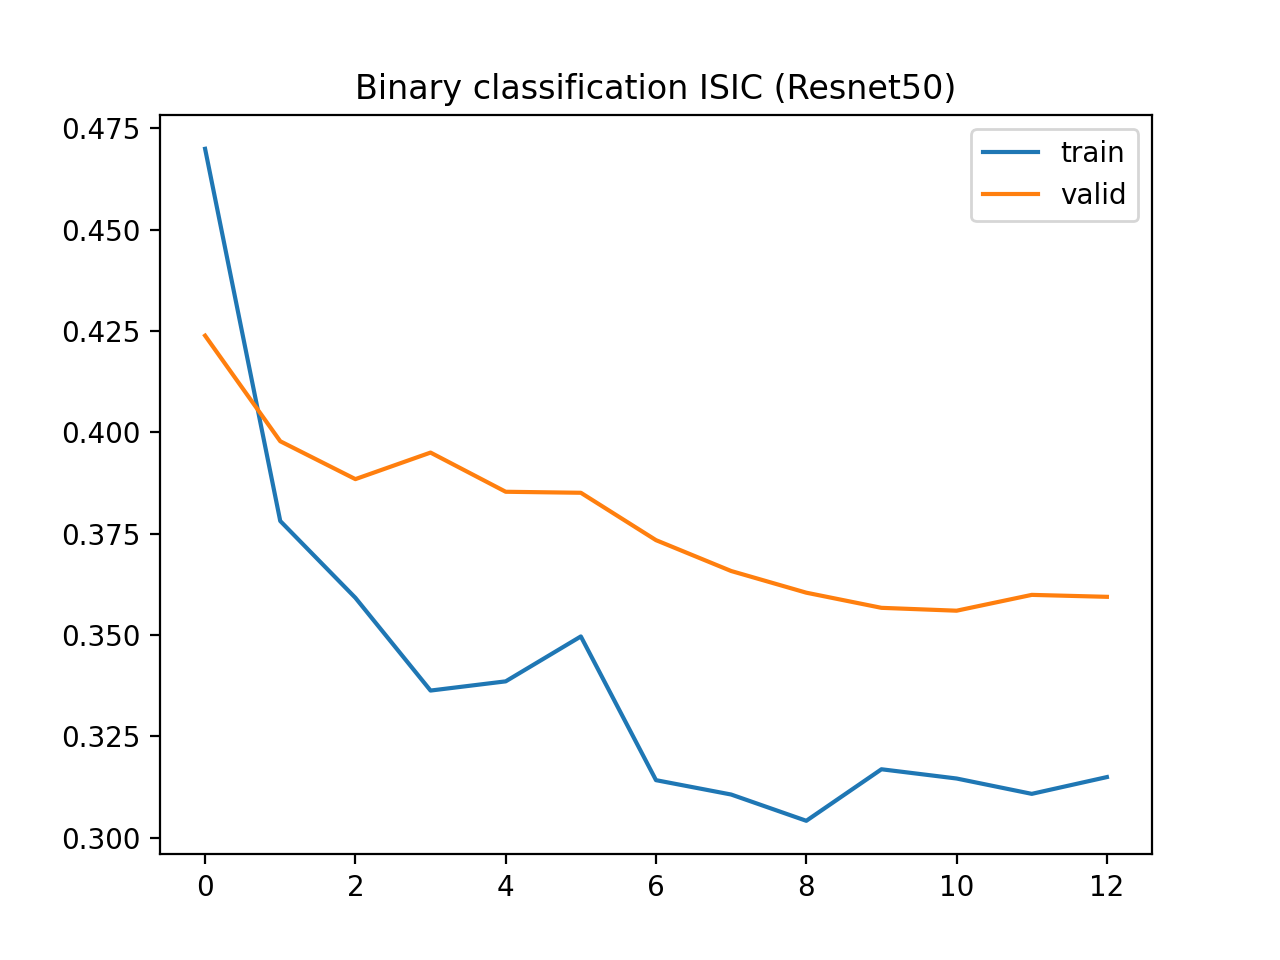
\includegraphics[width=0.45\textwidth]{imagenes/bin_class_resnetfreeze.png}} 
	\subfigure[Descongelado]{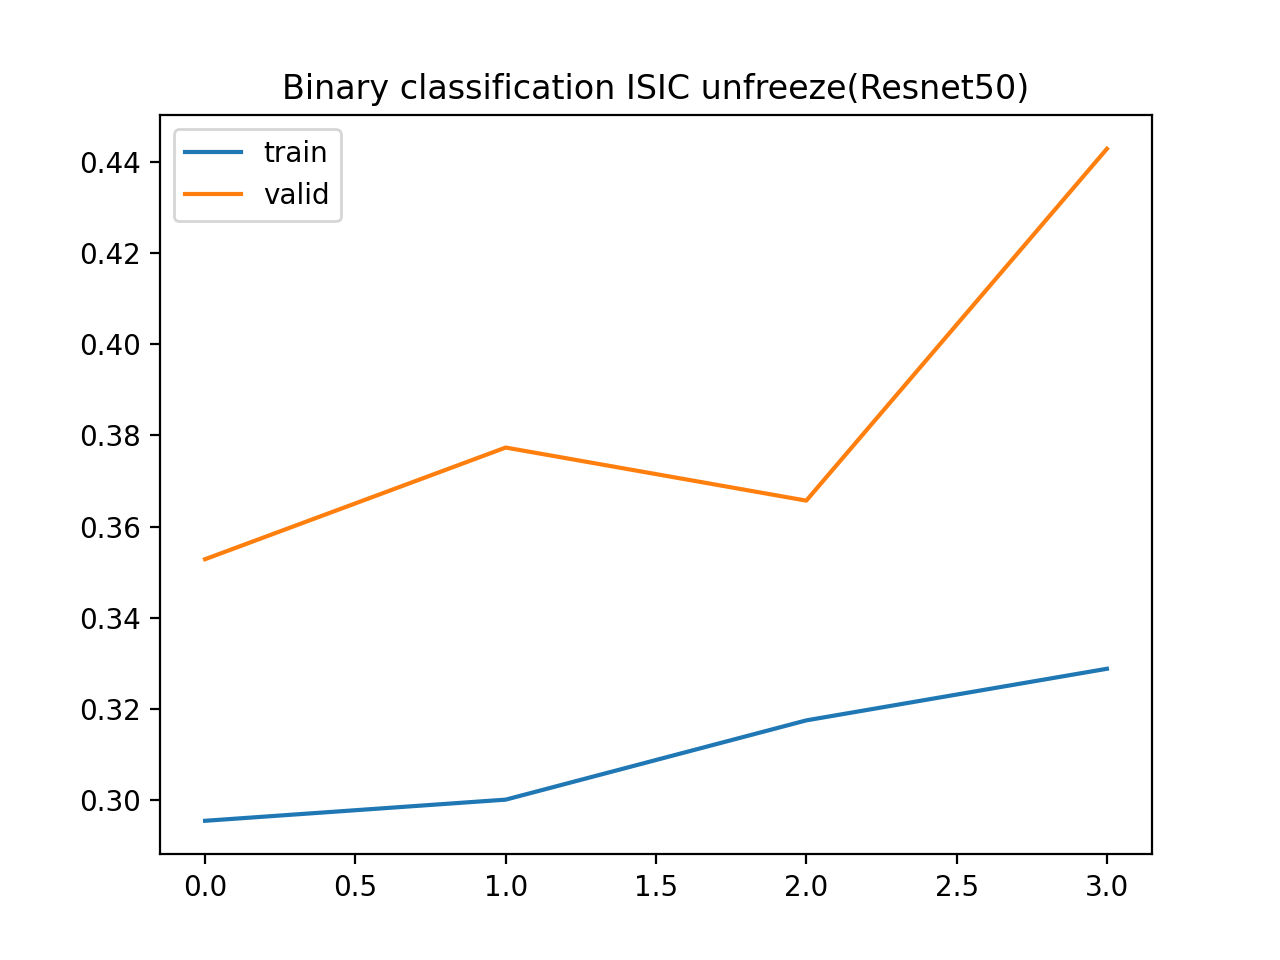
\includegraphics[width=0.45\textwidth]{imagenes/bin_class_resnetunfreeze.png}} 
	\caption{Curvas del finetuning del modelo binario con Resnet50}
	\label{fig:curvasrensetbinaria}
	
\end{figure}

A partir de dicha época, podemos apreciar un punto claro de inflexión de la curva, donde los valores de validación se disparan, alejándose de la curva de entrenamiento. Esto es detectado por el callback de Early Stopping, el cual cancela el entrenamiento al detectar un empeoramiento en 3 épocas continuas. En resumen, podemos concluir que el entrenamiento durante la fase de congelado se ha realizado correctamente.

En la segunda fase del proceso de finetuning, la fase de descongelado, los resultados no han sido tan positivos; el modelo sólo ha conseguido mejorar durante las dos primeras épocas, y las tres últimas han supuesto un empeoramiento que ha provocado la activación del early stopping en la quinta época. Si bien los resultados no han supuesto grandes mejoras, este comportamiento denota la complejidad que posee el modelo completo descongelado, y lo adecuadamente afinado que ya se encontraba gracias al preentrenamiento de la red con ImageNet.\\

A modo de referencia para comparación de los dos siguientes modelos a probar, este modelo ha requerido 4 horas y media para el proceso de entrenamiento, y 1.65 horas para el proceso de oversampling de la clase minoritaria, que ha llegado a ocupar 240GB de disco. Sin embargo, este último proceso sólo ha sido realizado para esta primera prueba, y el resto de modelos utilizarán este conjunto ya configurado.\\

En conclusión, la técnica de oversampling ha dado sus frutos, y hemos conseguido una mejora significativa en las métricas de la clase minoritaria sin afectar negativamente a la mayoritaria. A continuación, probaremos otros dos modelos para seleccionar el que exhiba mejor comportamiento.

\subsubsection{Efficient Net}

EfficientNet B5 es la segunda arquitectura elegida para su comparación. Esta arquitectura es el modelo más profundo de los 3 evaluados, por lo que los resultados han de ser considerablemente mejores para que se justifique la mayor complejidad. Aplicando el mismo conjunto de datos con oversampling creado para el entrenamiento de ResNet50, el resultado obtenido puede apreciarse en la tabla \ref{tab:resefnet}.

\begin{table}[H]
	\centering
	\begin{tabular}{|c|c|c|c|c|}
		\hline
		\textbf{} & \textbf{Precision} & \textbf{Recall} & \textbf{F1-score} & \textbf{Support} \\ \hline
		\textbf{Benign} & 0.89 & 0.93 & 0.91 & 7205 \\ \hline
		\textbf{Malignant} & 0.76 & 0.65 & 0.70 & 2460 \\ \hline
		\textbf{Accuracy} &  &  & 0.86 & 9665 \\ \hline
		\textbf{Macro avg} & 0.83& 0.79 & 0.8 & 9665 \\ \hline
		\textbf{Weighted avg} & 0.85 & 0.83 & 0.86 & 9665 \\ \hline
	\end{tabular}
	\caption{Informe de clasificación de EfficientNet B5}
	\label{tab:resefnet}
\end{table}

A la vista de los resultados, podemos apreciar que se produce una mejora en las métricas obtenidas en lo que respecta a accuracy, pero las métricas de precision y recall tienden a ofrecer mejores resultados para la clase mayoritaria. La tasa de aciertos para ambas clases ( accuracy) ronda el valor de 0.85, que se traduce en iun 85\% de los casos correctamente clasificados.  Sin embargo, si analizamos las curvas de aprendizaje \ref{fig:curvasefnetbinaria}, podemos observar un fenómeno llamativo: la curva no sigue la tendencia habitual a minimizarse, y existen crecidas repentinas de la función, dando lugar a picos de error:

l\begin{figure}[H]
	\centering
	\subfigure[Fase de congelado]{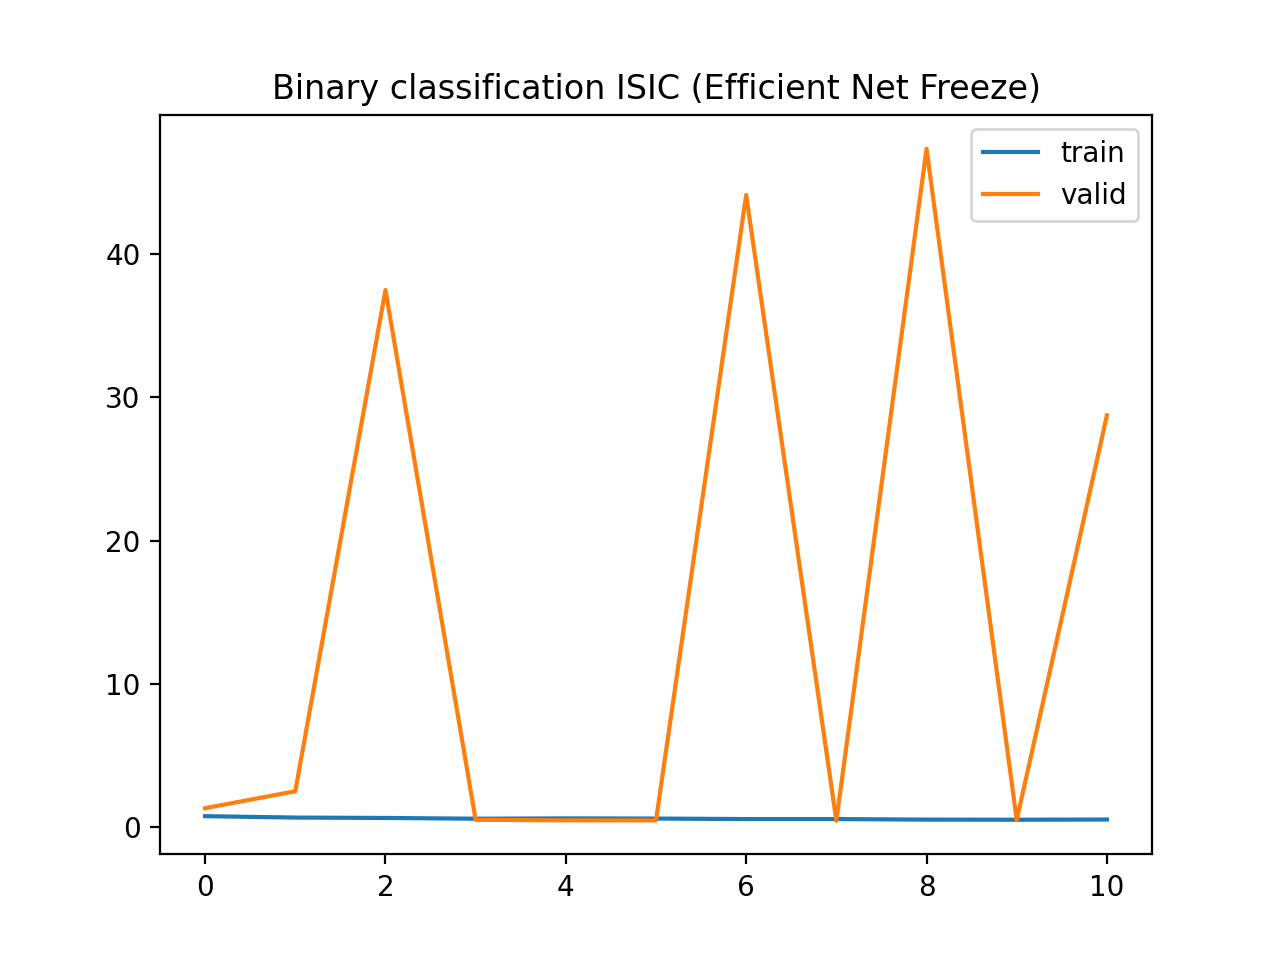
\includegraphics[width=0.45\textwidth]{imagenes/bin_class_efnetfreeze.png}} 
	\subfigure[Descongelado]{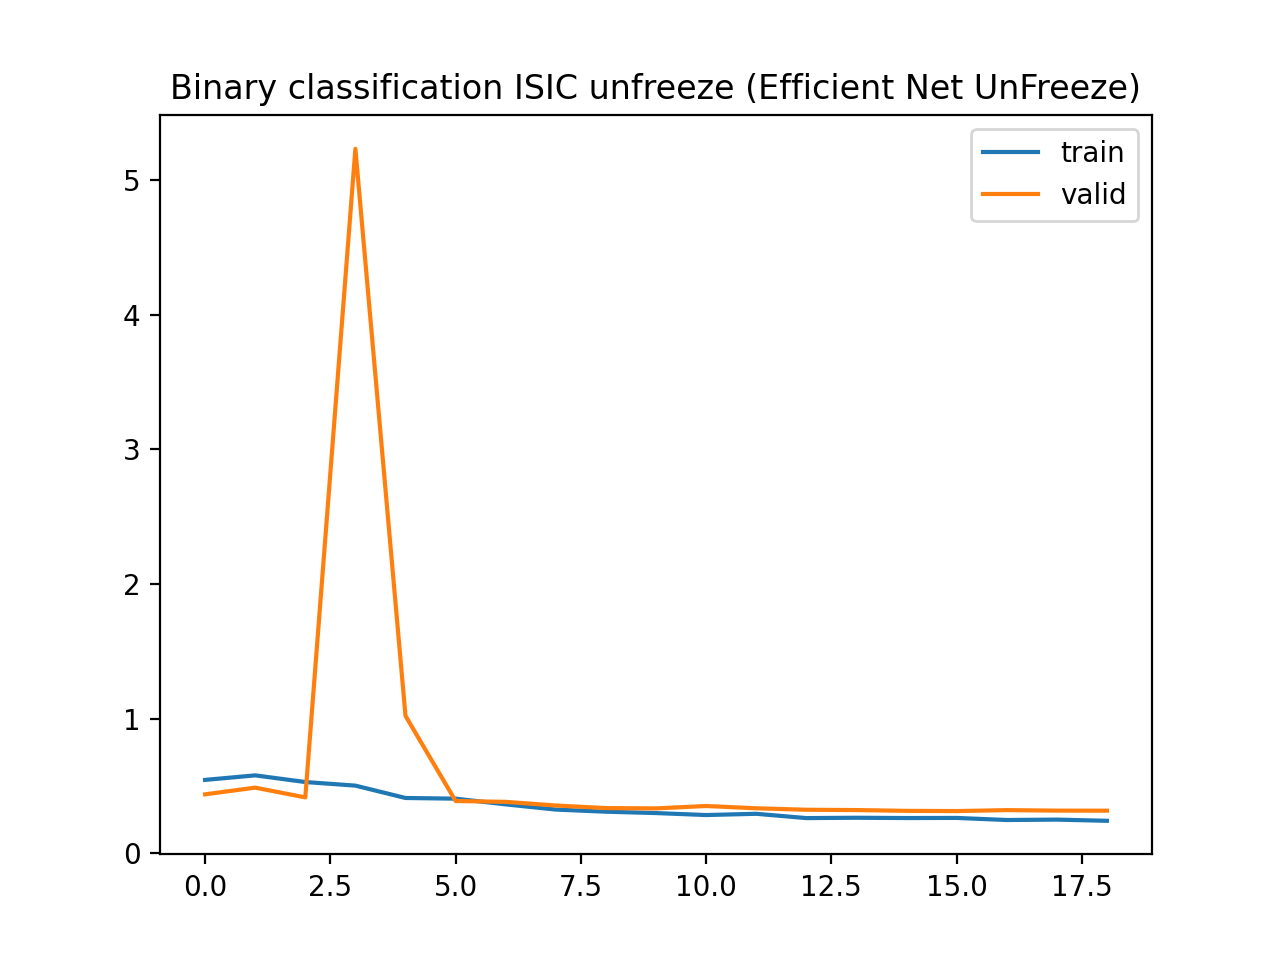
\includegraphics[width=0.45\textwidth]{imagenes/bin_class_efnetunfreeze.png}} 
	\caption{Curvas del finetuning del modelo binario con EfficientNet B5}
	\label{fig:curvasefnetbinaria}
\end{figure}

Este fenómeno puede deberse al reajuste de pesos fruto del learning rate variable, donde un subconjunto de las imágenes correctamente etiquetadas es cambiada de clase a la hora de modificar los valores para adaptarse a otro conjunto distinto no correctamente clasificado hasta el momento. También puede tratarse de un mal ajuste del learning rate, pero esto no es posible al utilzar la política de un ciclo con learning rate adaptativo.\\

Este fenómeno, de forma aislada, no supone ningún problema destacable sobre el entrenamiento, pero en este caso, observamos  cierta periodicidad en el fenómeno que lo convierte en un comportamiento preocupante.

Curiosamente, este fenómeno no se ve reflejado de la misma forma en la fase de descongelado del modelo; a diferencia de Resnet, el modelo si ha mejorado considerablemente en esta fase, aunque la tendencia descendente de la curva se ve eclipsada por el pico obtenido en la época número 3. En este caso, sí que podríamos considerar el pico como un fenómeno aislado sin mayor importancia.

 En este modelo, el tiempo de aprendizaje ha sido de aproximademante 7.7 horas, pero ha requerido el reinicio del entrenamiento en 5 ocasiones. Dichos problemas, asociados principalmente al desbordamiento de la memoria de GPU, y la precisión de los tensores, denota que el entrenamiento de este modelo no se ha realizado en condiciones óptimas, siendo uno de los factores posibles la necesidad de una mayor memoria de GPU. Por tanto, los resultados de este modelo han de considerarse con cautela, ya que la inestabilidad del entrenamiento y el aumento considerable de coste computacional lo convierten en una alternativa menos atractiva.

\subsubsection{Mobile Net}

MobileNet es el tercer modelo a evaluar con el conjunto de entrenamiento con sobremuestreo. Se trata del modelo con menor número de parámetros y profundidad, por lo que no se esperan mejores resultados en lo que respecta  a la métrica. Sin embargo, su simplicidad, especialmente dedicada para dispositivos de baja potencia, puede convertirse en una gran ventaja si los resultados no se ven considerablemente penalizados.\\

Tras realizar el entrenamiento, los resultados obtenidos por el conjunto de validación, nuestro estimador, son los mostrados en la tabla \ref{tab:mob}, donde, como era de esperar, no apreciamos mejores resultados en cuanto a métricas:   

\begin{table}[H]
	\centering
	\begin{tabular}{|c|c|c|c|c|}
		\hline
		\textbf{} & \textbf{Precision} & \textbf{Recall} & \textbf{F1-score} & \textbf{Support} \\ \hline
		\textbf{Benign} & 0.87 & 0.86 & 0.86 & 7205 \\ \hline
		\textbf{Malignant} & 0.60 & 0.61 & 0.60 & 2460 \\ \hline
		\textbf{Accuracy} &  &  & 0.80 & 9665 \\ \hline
		\textbf{Macro avg} & 0.73 & 0.74 & 0.73 & 9665 \\ \hline
		\textbf{Weighted avg} & 0.80& 0.80 & 0.80 & 9665 \\ \hline
	\end{tabular}
	\caption{Informe de clasificación de EfficientNet B5}
	\label{tab:mob}
\end{table}

A la vista de los resultados, podemos apreciar como la métrica especialmente penalizada es la columna de precision, donde la diferencia con los modelos anteriores es superior a una décima. Tratándose de la clase minoritaria, es un factor clave que este valor sea lo más alto posible para evitar casos malignos incorrectamente clasificados como benignos. El coste de una enfermedad maligna mal clasificada es superior al de una benigna, por lo que en cuanto a resultados, no se trata de un modelo que destaque. Sin embargo, su reducido tamaño, aproximadamente 4 veces menor que ResNet, lo haría una opción interesante para dispositivos de escaso potencia y con requisitos de bajo consumo.

Si estudiamos las curvas de aprendizaje (figura \ref{fig:curvasmbin}), se puede apreciar un comportamiento prácticamente ideal de la función  de pérdida de validación con respecto a entrenamiento; en la fase de congelado tanto el estimador de la pérdida en la función de entrenamiento como el de validación progresan en un intervalo de valores muy similares, sin picos bruscos, y con tendencia descendente. Como aspecto destacable, podemos observar cierto aplanamiento del modelo, y sin tendencia clara de sobreaprendizaje. Esto significa que el modelo ha alcanzado su límite de optimización, y debido a su arquitectura poco profunda, no es capaz de obtener valores más cercanos a la función real al disponer de menor dimensionalidad.

En la fase de descongelado, el resultado obtenido no es para nada similar a la tendencia de entrenamiento: obtenemos una aprendizaje muy ruidoso, con gran cantidad de picos y oscilaciones. Además, existe una tendencia clara de aumento de la función de pérdida en entrenamiento, lo cual refleja, en conjunto, que se está produciendo sobreaprendizaje. Por este motivo, en la cuarta época finaliza el entrenamiento, y se conservan los valores de la fase de congelado al haber empeorado los resultados en todas las épocas.

l\begin{figure}[H]
	\centering
	\subfigure[Fase de congelado]{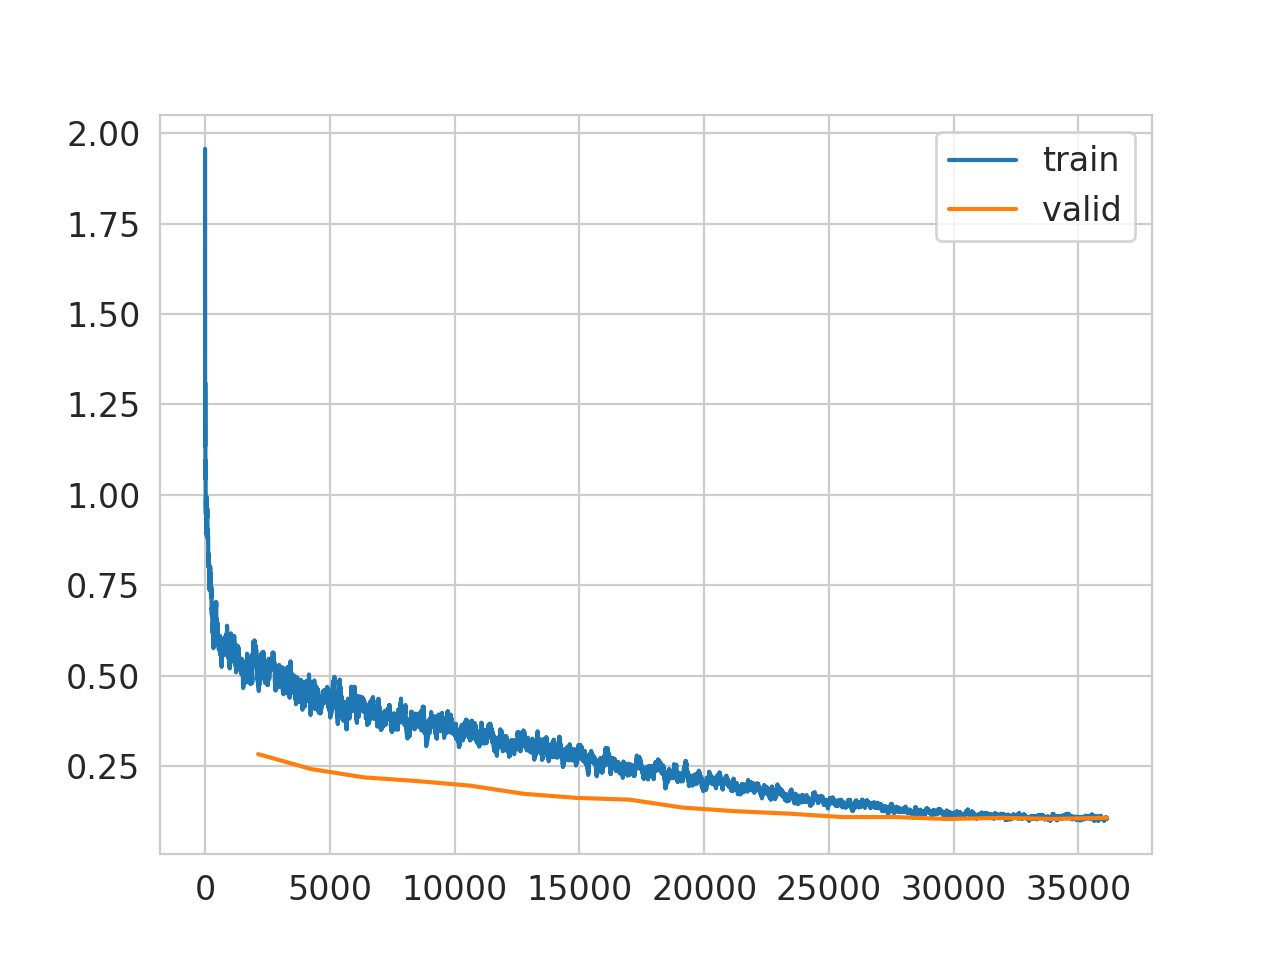
\includegraphics[width=0.45\textwidth]{imagenes/perdidasmobv2_freeze_equilib.png}} 
	\subfigure[Descongelado]{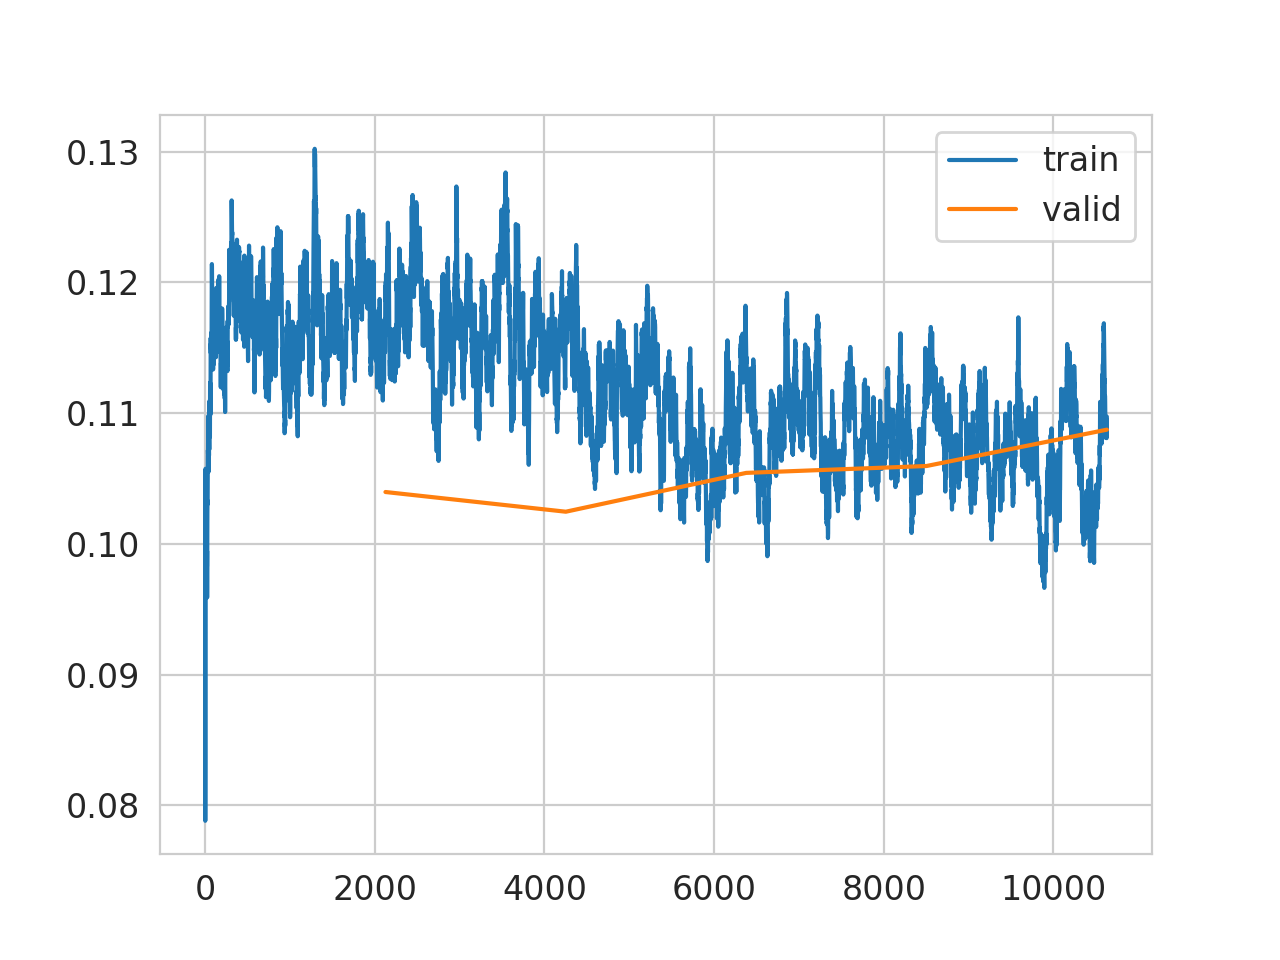
\includegraphics[width=0.45\textwidth]{imagenes/perdidasmobv2_unfreeze_equilib.png}} 
	\caption{Curvas del finetuning del modelo binario con Mobilenet V2}
	\label{fig:curvasmbin}
\end{figure}

En resumen, se trata de un modelo fácilmente entrenable, con apenas 2.18 horas de entrenamiento, pero con capacidades de cálculo bastante limitadas.

\subsection{Modelo seleccionado}

Tras el entrenamiento de los 3 modelos, y su correspondiente evaluación mediante el conjunto de validación, es posible tomar la decisión de qué modelo emplear para realizar la cuantización del modelo. Para ello, de la forma tradicional, bastaría con mirar la tabla de resultados de forma conjunta, y elegir aquel que demuestre un mejor resultado promedio en las métricas obtenidas. Pero, en este caso, tendré en cuenta otros factores, como la calidad de las curvas de aprendizaje, el número parámetros como medida de complejidad del modelo (junto a su número de capas), y el tiempo empleado para la inferencia, y de forma consecuente, para el entrenamiento.

Siguiendo el primer criterio, las métricas, el claro ganador en cuanto a tasa de aciertos se refiere es EfficientNet, ya que su valoración para la métrica balanced accuracy es del 81\%. Sin embargo, si atendemos al resto de valores, podemos apreciar que ResNet50 ofrece resultados bastante cercanos,  requiriendo casi la mitad de tiempo para alcanzar este resultado con respecto a EfficientNet.


\begin{table}[H]
	\centering
	\begin{tabular}{|c|c|c|c|c|}
		\hline
		\textbf{Modelo} & \textbf{Precision} & \textbf{Recall} & \textbf{Accuracy} & \textbf{Bal. Accuracy} \\ \hline
		EfficientNet B5 & 0.83 & 0.79 & 0.86 & 0.82 \\ \hline
		Resnet50 & 0.79 & 0.79 & 0.84 & 0.80 \\ \hline
		MobileNet V2 & 0.74 & 0.73 & 0.8 & 0.74 \\ \hline
	\end{tabular}
	\caption{Valores de las métricas de cada modelo}
	\label {fig:metricas}
\end{table}

Además, Resnet ofrece resultados equilibrados en todas sus métricas, mientras EfficientNet aprece destaar especialmente en precision, aunque se igualan en recall.

MobileNet, por su parte, ofrece resultados distantes de los dos modelos anteriores, debido, a como ya se mencionó, su menor profundidad y capacidad expresiva para su ejecución en entornos ligeros. Aunque los resultados no son demasiado lejanos a ResNet, considero que este último es una mejor alternativa para el problema que estamos desarrollando.\\

Aunque a su vez, Resnet se trata de un peor modelo comparado con EfficientNet a nivel de métricas, el aprendizaje ofrecido por EfficientNet es bastante confuso por la existencia de los picos ya mostrados anteriormente. Debido a la periodicidad de los mismos, el coste computacional adicional, y los errores por falta de recursos ya producidos sin realizar cuantización, considero que no se trata de una buena alternativa, y que Resnet50 es el modelo indicado para este problema.\\

La complejidad adicional de EfficientNet en cuanto a sus parámetros de anchura, entrada y profundidad, así como su mayor cantidad de parámetros y capas de profundidad variable, lo convierten en un modelo demasiado complejo. Sin medimos el tamaño de cada modelo una vez exportado, obtenemos los siguientes valores: 

\begin{figure}[H]
	\centering
	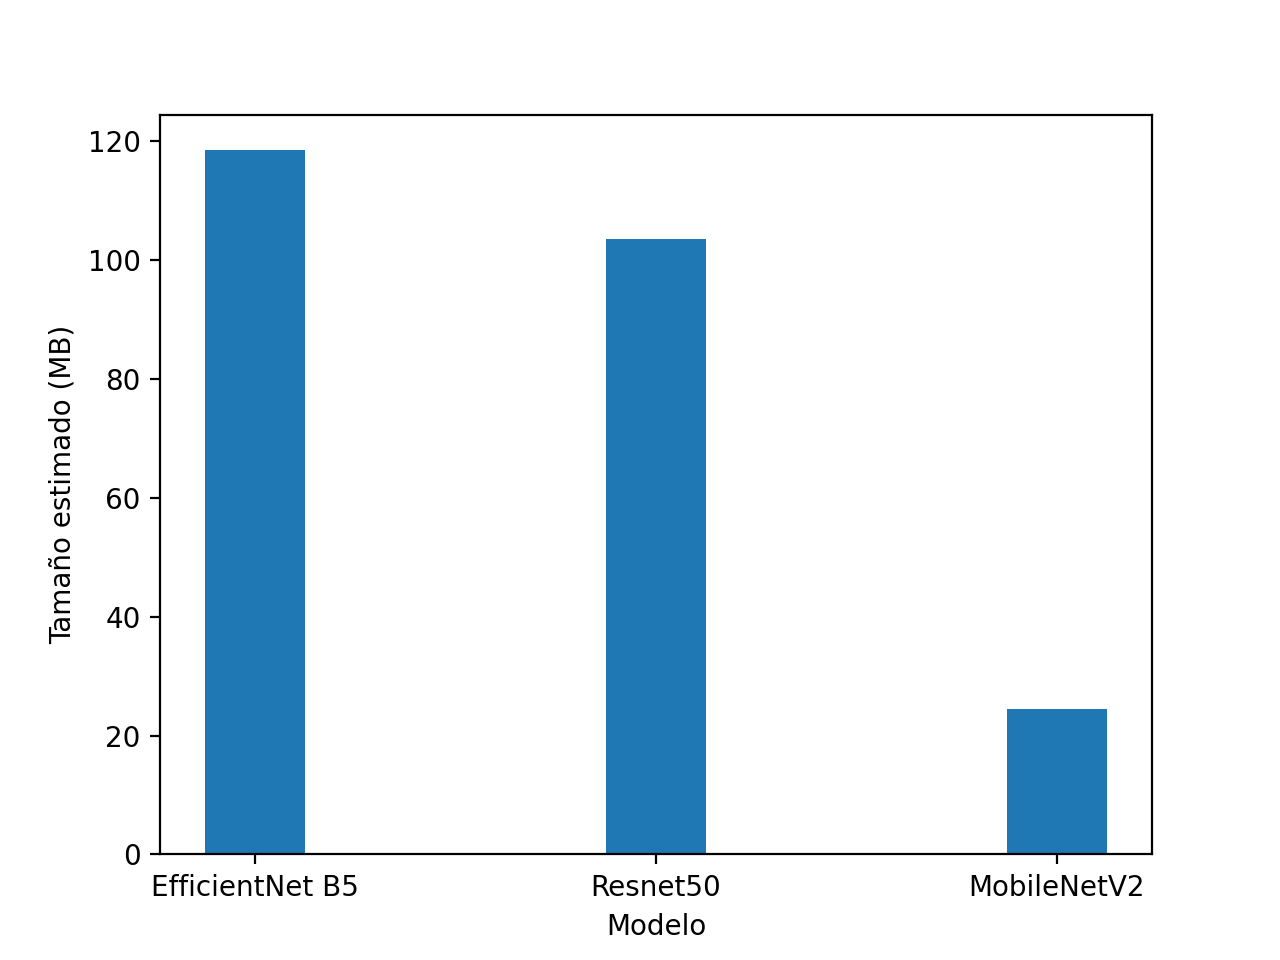
\includegraphics[scale = 0.6]{imagenes/tamestimado.png}
	\caption{Espacio (en MB) requerido por cada modelo}
	\label {fig:tam}
\end{figure}

Por tanto, realizaremos el proceso de cuantizado con Resnet, ya que dará lugar a un modelo más versatil al ser cuantizado, y tiene expresividad de cálculo suficiente para el problema de clasificación multiclase. Además, ofrecerá un mejor resultado en rendimiento de inferencia que EfficientNet en dispositivos móviles.


\section {Clasificación multiclase}

Una vez distinguida si la enfermedad de entrada es benigna o maligna, debemos de indicar de qué tipo de enfermedad se trata.  Como ya enunciamos en los objetivos de este proyecto, el proposito  del mismo consiste en crear una arquitectura de dos modelos, donde primero, se establece si la enfermedad es benigna o maligna, y posteriormente, se clasifica la posible enfermedad de la que se trata. De esta forma, podemos modularizar el espacio, y entrenar ambos modelos por separado de forma paralela si fuera necesario.

De esta fase de entrenamiento, obtendremos dos modelos distintos, compeltamente aislados entre sí: uno de ellos, dedicado a las enfermedades malignas, y otro, únicamente a las benignas. El proceso a seguir será exactamente el mismo que con clasificación binaria: creación del dataset, entrenamiento, y evaluación del conjunto de validación.

En este caso, no se aplicará oversampling para mostrar las clases en su correspondiente proporción real.  Además, debido a los grandes desequilibrios existentes entre clase, sería imposible igualar en número todas las clases a clasificar, y ocuparía un espacio en disco del cual no se dispone para la realización del proyecto.

\subsection{Modelo de enfermedades malignas}

Comenzaremos por las imágenes malignas. En este caso, al estar utilizando finalmente únicamente el conjunto de entrenamiento de ISIC, disponemos de 4 clases diferenciadas:

\begin{itemize}
	\item Basal cell carcinoma
	\item Melanoma
	\item Melanoma metastasis
	\item Squamous cell carcinoma
	
\end{itemize}

Dichas clases poseen un desbalanceo considerable. La clase menos representada se trata de los melanomas metastásicos, que representa solo el 0.22 \% del total de datos malignos. Como una clase con dicha proporción no se puede clasificar adecuadamente, aprovecharemos la existencia de la clase melanoma para introducir sus ejemplos como parte de esta clase, dando lugar a una nueva distribución (figura \ref{fig:malas}). Esta fusión es posible debido a que ambas clases representan la misma enfermedad, pero siendo la metastasis una fase más avanzada, y con baja tasa de supervivencia por su diseminación a otros órganos vitales.

\begin{figure}[H]
	\centering
	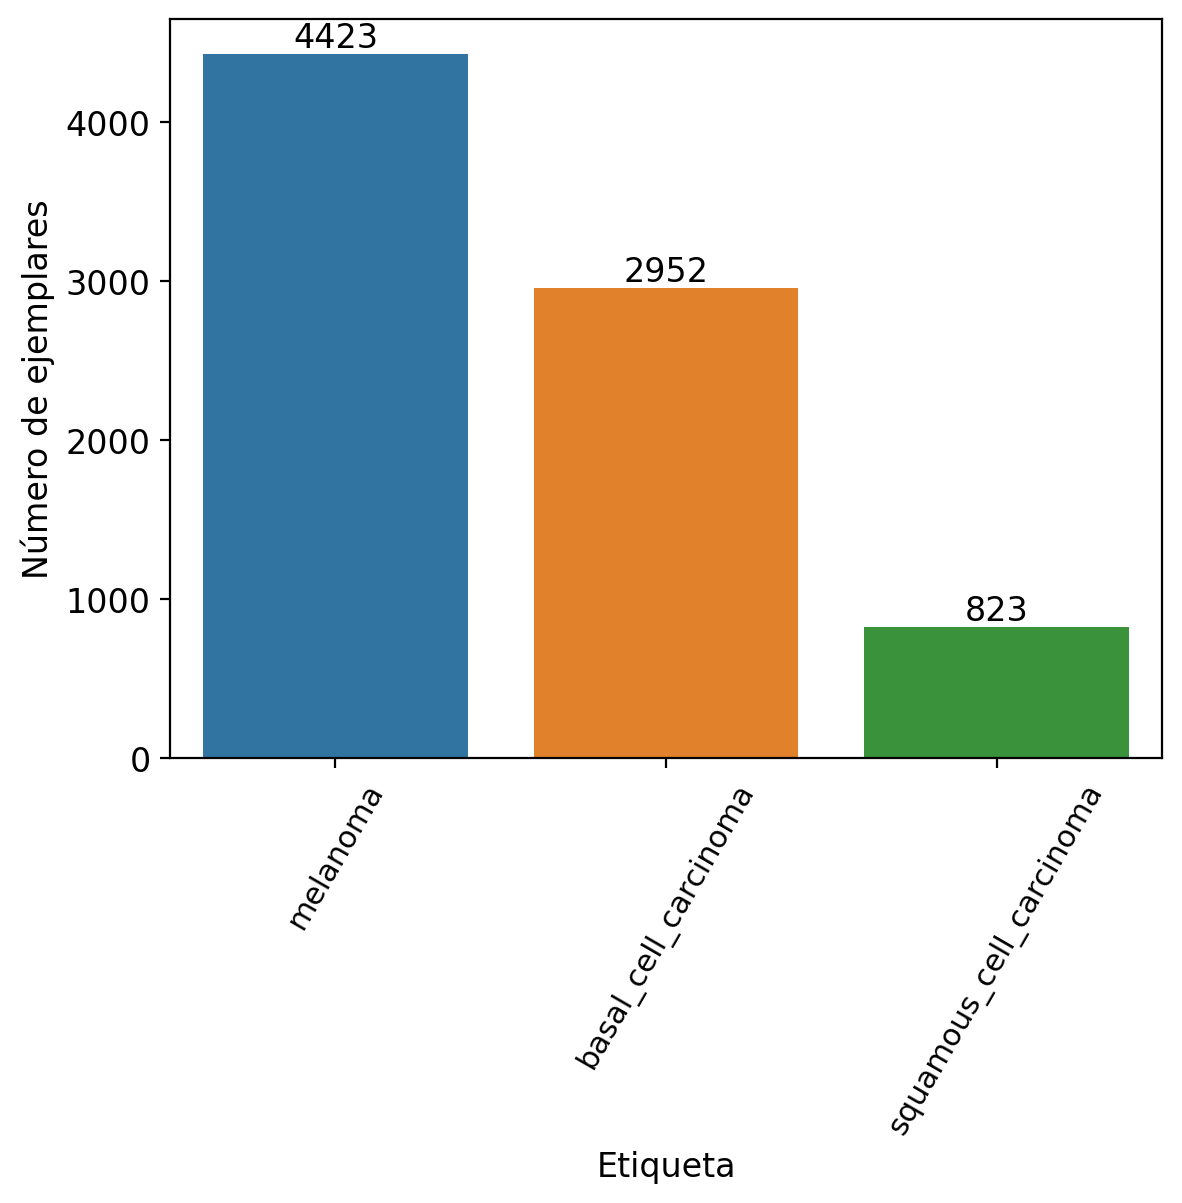
\includegraphics[scale = 0.6]{imagenes/countmalignant.png}
	\caption{Distribución de las clases malignas}
	\label {fig:malas}
\end{figure}


Al realizar esta acción, aumentamos el número de ejemplares de la clase mayoritaria, pero se trata de una situación preferible sobre la exitencia de una clase minoritaria, ya que ésta penalizará considerablemente las métricas al ser todas ellas métricas equlibradas según la proproción de imágenes de cada clase.

\subsubsection{Entrenamiento}

Para el entrenamiento del modelo, haré uso de la misma configuración que la clasificación binaria: imágenes 512 x 512, tamaño de batch de 32, pero con la diferencia de no emplear oversamplin por las razones ya explicadas. Si representamos al anterior gráfico de barras \ref{fig:malas} como proporciones porcentuales, obtenemos una distribución notablemente desequilibrada:

\begin{itemize}
	\item Melanoma: 53.95\%
	\item Células basales: 36\%
	\item Células escamosas: 10.5\%
 \end{itemize}
 
 Dichas clases, a pesar del desbalanceo, poseen una representatividad suficiente como para ser clasificadas en conjunto de forma adecuada. Para la clasificación, esta vez haremos uso de la función de pérdida FocalLoss, gracias a su capacidad de equilibrar el entrenamiento mediante el uso de sus parámetros $\alpha = 0.25$ y $\gamma = 2$, que son los valores recomendados por su paper original \cite{lin2018focal}.
 
 Tras el entrenamiento, se han obtenido las métricas referenciadas en la tabla \ref{tab:malignometrics}. Podemos apreciar una valoración positiva de las métricas, ya que para Basal Cell carcinoma y los melanomas, precision y recall adquieren valores superiores a 0.8, acercándose a 0.9 en precisión y 0.92 de recall en melanomas.  La clase minoritaria de las 3, Squamous cell carcinoma, tiene un recall bajo, cercano a 0.4, mientras que una precisión algo más notable de 0.66.

\begin{table}[!ht]
	\centering
	\begin{tabular}{|l|c|c|c|c|}
		\hline
		& Precision & Recall & F1-score & Support \\
		\hline
		Basal cell & 0.81 & 0.85 & 0.83 & 908 \\
		Melanoma & 0.88 & 0.92 & 0.90 & 1311 \\
		Squamous cell & 0.66 & 0.38 & 0.48 & 240 \\
		\hline
		Accuracy &  &  & 0.84 & 19464 \\
		Macro avg & 0.79& 0.72& 0.74&2459\\
		Weighted avg&0.84&0.84&0.84&2459\\
		\hline
	\end{tabular}
	\caption{Informe de clasificación para validación maligna}
	\label{tab:malignometrics}
\end{table}

Aunque se traten de resultados negativos para la clase minoritaria, el conjunto del modelo ofrece resultados  adecuados, con una precisión de casi 80\%, y un 72\% de recall, que arrojan un resultado final de 84\% de accuracy. Si observamos las curvas de aprendizaje (figura \ref{fig:curvasmalign} ), el comportamiento de la función de pérdida denota un correcto aprendizaje en la fase de congelado del modelo.

l\begin{figure}[H]
	\centering
	\subfigure[Fase de congelado]{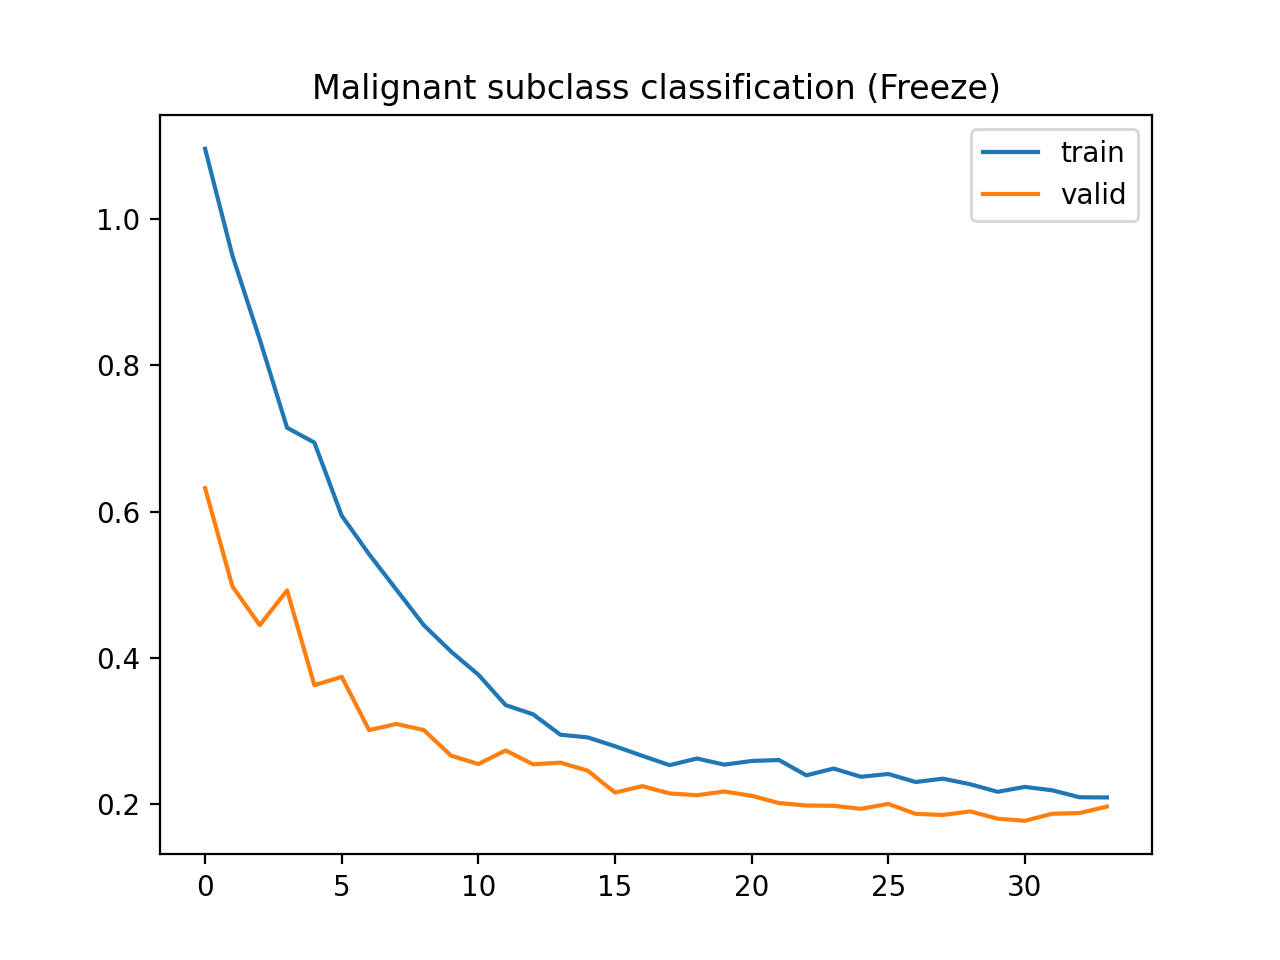
\includegraphics[width=0.475\textwidth]{imagenes/malignant_freeze.png}} 
	\subfigure[Descongelado]{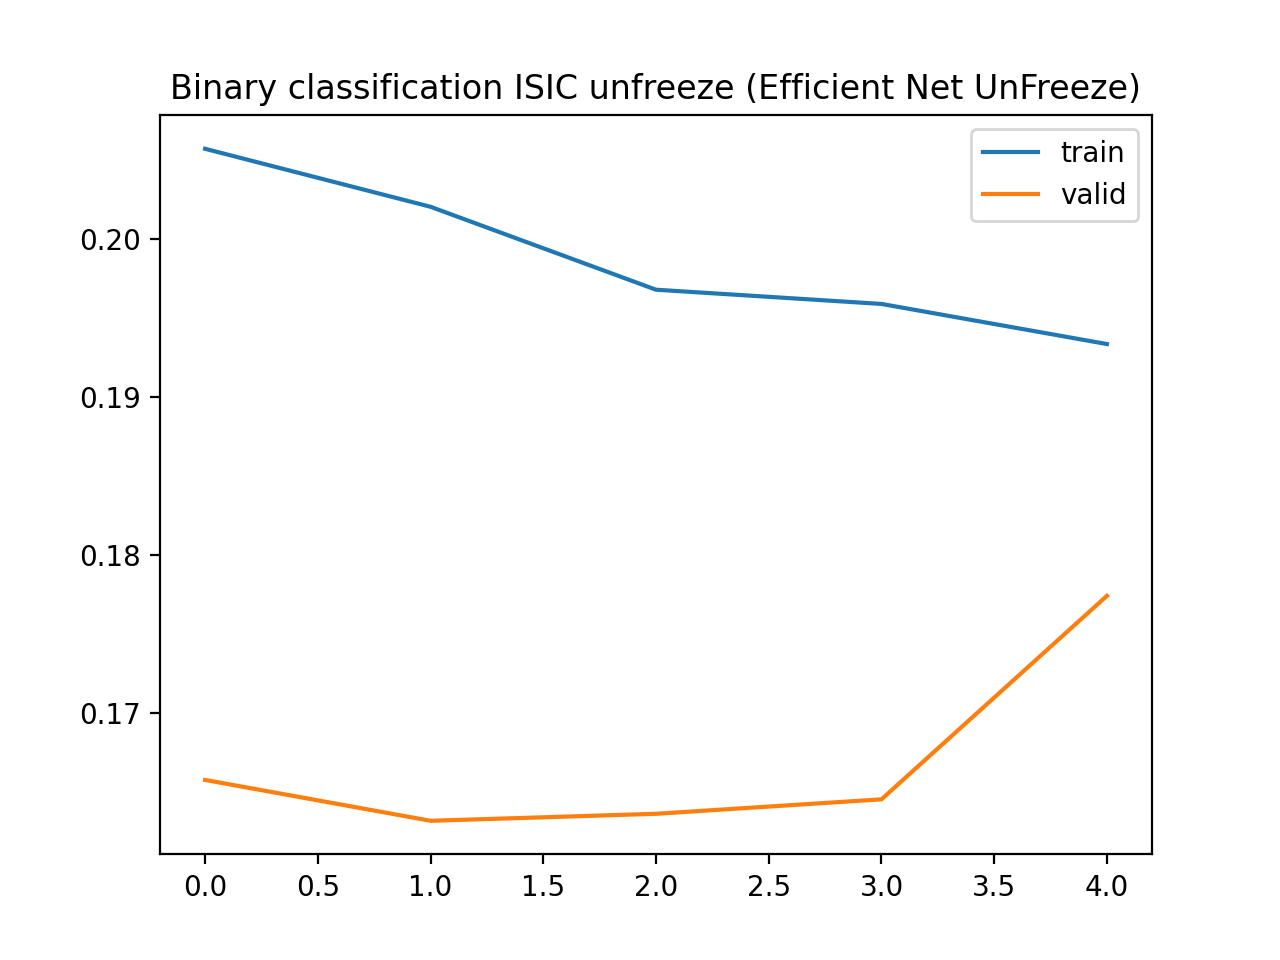
\includegraphics[width=0.475\textwidth]{imagenes/malignant_unfreeze.png}} 
	\caption{Curvas de aprendizaje para clases malignas}
	\label{fig:curvasmalign}
\end{figure}

Podemos observar como, a diferencia del resto de modelos evaluados hasta el momento, la curva de aprendizaje para el conjunto de validación permanece por debajo de la curva de aprendizaje. Esto no significa que el proceso de entrenamiento sea incorrecto: se debe a un efecto del aumento de datos, y la aplicación de Focal Loss. Al unir ambos mecanismos, estamos provocando que la evaluación del conjunto de entrenamiento sea más compleja que validación, ya que en validación solo se realiza un inferencia de las imágenes, pero entrenamiento es utilizado continuamente para reajustar la función, y fomentar la correcta clasificación de aquellos elementos ``dificiles de clasificar''. Se trata de un efecto no negativo, y el entrenamiento se ha realizado satisfactoriamente.

No podemos afirmar lo mismo de la fase de descogenlado, ya que tras realizar cinco épocas se ha alcanzando overfitting del modelo, ya que el callback de Early Stopping ha cancelado el entrenamiento antes del límite de épocas establecido (el cual, si recordamos, se trataba de un valor alto para que early stopping decidiera cuando realizar la parada). Por tanto, los resultados obtenidos en la segunda fase son prácticamente descartables, y no han ofrecido valor ninguno al modelo final.

En resumen, el modelo obtenido cumple adecuadamente los requisitos del problema. Sin embargo, como forma de evaluar si eran posibles mejores resultados, se realizó un segundo entrenamiento, aplicando pesos a la función de pérdida para penalizar en mayor medida incorrectas clasificaciones de la clase minoritaria. Basta con aplicar la siguiente operación, donde, considerando el valor c como el número de ejemplares de la clase C:

$$p_C =(\frac{c}{\sum_{i=0}^{num\_clases} c} )^{-1}$$

De esta forma, haremos que cada ejemplar tenga un peso acorde a su proproción en el dataset. Si repetimos el experimento siguiendo este razonamiento, obtenemos los siguientes resultados:

\begin{table}[!ht]
	\centering
	\begin{tabular}{|l|c|c|c|c|}
		\hline
		& Precision & Recall & F1-score & Support \\
		\hline
		Basal cell & 0.66 & 0.66 & 0.66 & 908 \\
		Melanoma & 0.83 & 0.76 & 0.79 & 1311 \\
		Squamous cell & 0.30 & 0.42 & 0.35 & 240 \\
		\hline
		Accuracy &  &  & 0.69 & 19464 \\
		Macro avg & 0.59& 0.62& 0.60&2459\\
		Weighted avg&0.71&0.69&0.70&2459\\
		\hline
	\end{tabular}
	\caption{Informe de clasificación para validación maligna (Pesos)}
	\label{tab:malignometrics2}
\end{table}


Donde, podemos observar que todas las métricas obtenidas son considerablemente inferiores a las de la versión inicial (\ref{tab:malignometrics}). Esto se debe a que, al insertar pesos a cada clase a clasificar, es altamente probable que se haya cancelado el efecto regularizador ofrecido por FocalLoss durante el entrenamiento.

Por tanto, podemos concluir de manera firme y justificada que el modelo entrenado anteriormente, sin ningún tipo de penalización adicional, y haciendo uso de Focal Loss, es el modelo adecuado para este subproblema.

\subsection{Modelo de enfermedades benignas}

Una vez entrenado el modelo correspondiente a las clases malignas, es el turno de construir el modelo de las clases benignas. Recordando el estudio realizado en el problema de clasificación binario, las clases benignas eran el subconjunto de datos dominante en el dataset. Esto se debe, principalmente, a que las lesiones cutáneas son frecuentemente lesiones no cancerosas. Disponemos de un conjunto de datos mucho más amplio, englobando 17 clases distintas.  Como es de esperar, la condición más frecuente de este conjunto son los lunares comunes, denominados nevus en dermatología.

El desbalanceo que se produce es un caso extremo, en cual la clase mayoritaria, el lunar común, engloba el 81\% del total, y el 19\% restante se reparte entre las 16 clases que restan (figura  \ref{fig:buenas}). Esto convierte al subproblema en un reto considerable de resolver con un modelo del tamaño de Resnet50, por lo que se tratará de hallar los mejores resultados pero teniendo en cuenta el sacrificio que supone emplear modelos más ligeros que sean cuantizables y ejecutables en Android.

Dado el desbalanceo, se probarán dos alternativas distintas: la aplicación de la métrica Focal Loss sin ajuste de pesos, y la creación de un modelo basado en pesos inversamente proporcionales al número de ejemplares en dicha clase junto a CrossEntropy.

Para simplificar la notación empleada en el etiquetado de las enfermedades, se usarán las siguientes abreviaturas en las tablas de resultados:
\begin{multiitem}
	\item Nevus: NV
	\item Seborreic keratosis: SEK 
	\item Actinic keratosis: AK            
	\item Pigmented benign keratosis: PBK 
	\item Solar lentigo: SL
	\item Dermatofibroma: DER 
	\item Vascular lesion: VL                        
	\item Lichenoid keratosis: LK
	\item Acrochordon: ACR
	\item Lentigo NOS: LN
	\item Atypical melanocytic proliferation: AMP
	\item Aimp                                     
	\item 	Wart                                     
	\item Angioma: ANG                               
	\item Lentigo simplex: LS
	\item 	Neurofibroma: NF
	\item 	Scar 
\end{multiitem}

\begin{figure}[H]
	\centering
	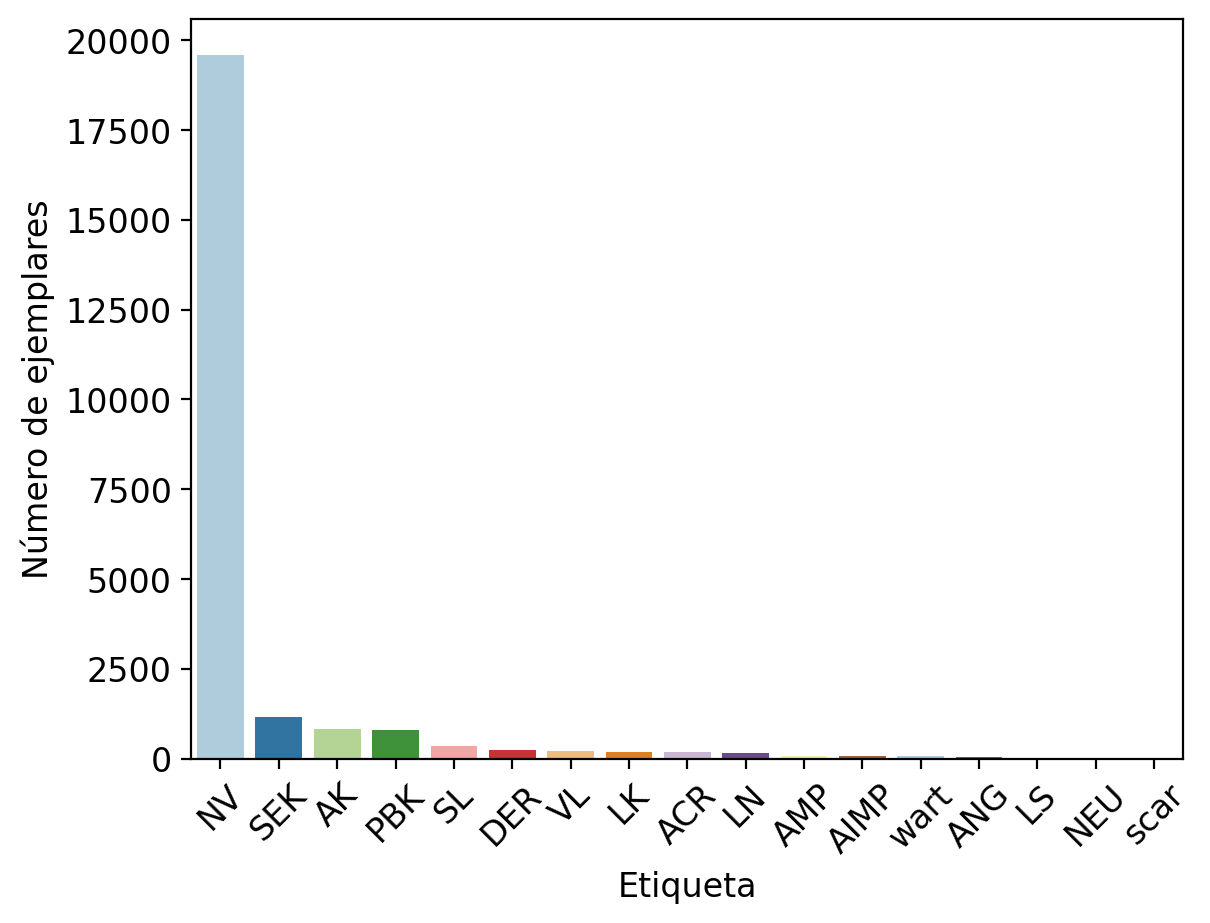
\includegraphics[scale = 0.7]{imagenes/countbenign.png}
	\caption{Conteo de clases benignas antes de agrupar}
	\label {fig:buenas}
\end{figure}

\subsubsection{Entrenamiento}

Conocemos que el desequilibrio del conjunto de entrenamiento es considerable. Pero, antes de probar otras soluciones más sofisticadas, es razonable considerar aplicar la misma técnica que la aplicada en clasificación binaria: el uso de la una métrica que tolere adecuadamente el desbalanceo, como FocalLoss.\\

Aplicando una configuración similar a la usada para el entrenamiento de las clases malignas, el resultado obtenido no esperanzador, y deja bastante que desear  (tabla \ref{tab:benignomalmetrics}). La clase de lunares comunes es la única que cuenta con métricas excelentes, ya que el resto de clases han sido clasificadas con valores de métrica bastante bajos. Si observamos los resultados,  los siguientes mejores casos provienen de los dermatofibromas, la queratosis benigna pigmenteada,  las lesiones vasculares, y la queratosis liquenoide. Estas obtienen unos valores de precision de 0.75, 0.71,0.68,0.67, respectivamente. Pero en el caso de recall, los dermatofibromas son ampliamente castigados, por lo que aunque la alta precisión nos aporta que el modelo es capaz de rechazar las clases que no lo son de manera aceptable, el recall bajo nos muestra que también los casos positivos están siendo identificados como negativos en la mayoría de casos.

\begin{table}[!ht]
	\centering
	\begin{tabular}{|l|c|c|c|c|}
		\hline
		& Precision & Recall & F1-score & Support \\
		\hline
		\textbf{NV} & 0.92 & 0.98 & 0.95 & 5864 \\ \hline
		\textbf{SK} & 0.50 & 0.35 & 0.41 & 345 \\ \hline
		\textbf{AK} & 0.53 & 0.58 & 0.56 & 265 \\ \hline
		\textbf{PBK} & 0.71 & 0.74 & 0.72 & 222 \\ \hline
		\textbf{SL} & 0.28 & 0.12 & 0.17 & 99 \\ \hline
		\textbf{DER} & 0.75 & 0.18 & 0.29 & 83 \\ \hline
		\textbf{VL} & 0.68 & 0.55 & 0.61 & 71 \\ \hline
		\textbf{LK} & 0.67 & 0.07 & 0.12 & 61 \\ \hline
		\textbf{ACR} & 0.46 & 0.24 & 0.32 & 54 \\ \hline
		\textbf{LN} & 0.16 & 0.11 & 0.13 & 44 \\ \hline
		\textbf{AMP} & 0.50 & 0.07 & 0.12 & 29 \\ \hline
		\textbf{AIMP} & 0.00 & 0.00 & 0.00 & 24 \\ \hline
		\textbf{WART} & 0.00 & 0.00 & 0.00 & 23 \\ \hline
		\textbf{ANG} & 0.29 & 0.33 & 0.31 & 6 \\ \hline
		\textbf{LS} & 0.00 & 0.00 & 0.00 & 5 \\ \hline
		\textbf{NEU} & 0.00 & 0.00 & 0.00 & 5 \\ \hline
		\textbf{SCAR} & 0.00 & 0.00 & 0.00 & 5 \\ \hline
		\hline
		Accuracy &  &  & 0.87 & 7205 \\
		Macro avg & 0.38& 0.25& 0.28&7205\\
		Weighted avg&0.84&0.87&0.85&7205\\
		\hline
	\end{tabular}
		\caption{Clasificación para validación benigna (Ordenadas de mayor a menor rep., sin pesos)}
	\label{tab:benignomalmetrics}
\end{table}

Esto ocurre en la mayoría de clases, aunque los peores resultados los vemos reflejados en las 6 últimas filas, donde 5 de las clases han sido completeamente ignoradas por el modelo, y establecidas a 0: la cicatrices, los neurofibromas, los lentigo simples, las verrugas y los AIMP (atypical intraepidermal melanocytic proliferation). Estas clases, al encontrarse en absoluta minoría, no aportan suficientes caracteristicas al modelo para aprender los filtros adecuados, y por tanto, quedan descartadas por el mismo. Esto nos lleva a tomar la decisión de descartar estas clases, o bien, tratar de equilibrarlas complementando con el resto de datasets.

No nos debemos dejar llevar por el valor del accuracy: este es del 87\%, debido a que prácticamente la completitud de la tasa de aciertos se ve aportada por la clase mayoritaria. Si atendemos a su valor medio, es del únicamente 28\%, que se trata de una cifra más representativa pero mucho más pesimista.

Para no proceder con la eliminación de clases minoritarias, trataremos de dotar al modelo de penalizaciones para las clases menos reprentadas; es decir, de forma explícita, estableceremos una serie de pesos que otorguen más importancia a clasificar ejemplares de clases minoritarias sobre las mayoritarias, calculando los pesos de la mismo forma en la que lo hicimos para el caso de las enfermedades malignas:

$$p_C =(\frac{c}{\sum_{i=0}^{num\_clases} c} )^{-1}$$

De esta forma, haremos que cada ejemplar tenga un peso acorde a su proproción en el dataset. La diferencia con el caso empleado en enfermeades malignas, es que emplearemos como función de pérdida CrossEntropy en lugar de FocalLoss, ya que pudimos apreciar en el caso anterior que al insertarle pesos, pierde el efecto regularizador visto en el caso sin pesos, y obtenemos peores resultados.

\begin{figure}[H]
	\centering
	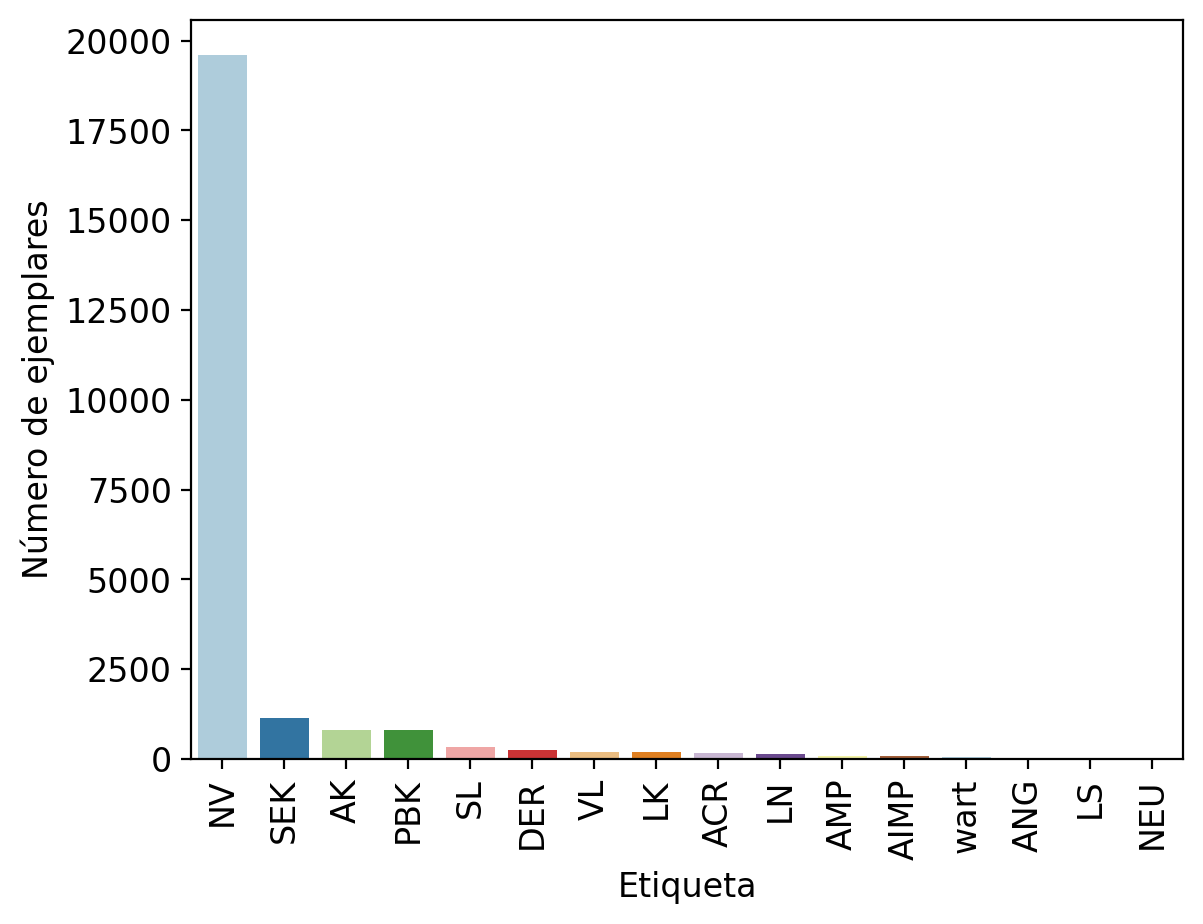
\includegraphics[scale = 0.7]{imagenes/countbenign_corrected.png}
	\caption{Conteo de clases benignas tras la agrupación}
	\label {fig:buenasred}
\end{figure}

De esta forma, si repetimos el experimento siguiendo este razonamiento, obtenemos los resultados de la tabla \ref{tab:benignomalmejormetrics}:


\begin{table}[!ht]
	\centering
	\begin{tabular}{|l|c|c|c|c|}
		\hline
		& Precision & Recall & F1-score & Support \\
		\hline
	\textbf{NV} & 0.99 & 0.77 & 0.86 & 5864 \\ \hline
	\textbf{DER} & 0.33 & 0.60 & 0.42 & 345 \\ \hline
	\textbf{PBK} & 0.53 & 0.59 & 0.56 & 265 \\ \hline
	\textbf{VL} & 0.37 & 0.88 & 0.52 & 222 \\ \hline
	\textbf{LK} & 0.18 & 0.46 & 0.26 & 99 \\ \hline
	\textbf{AK} & 0.31 & 0.63 & 0.41 & 83 \\ \hline
	\textbf{SK} & 0.58 & 0.83 & 0.69 & 71 \\ \hline
	\textbf{AMP} & 0.20 & 0.39 & 0.26 & 61 \\ \hline
	\textbf{ACR} & 0.23 & 0.67 & 0.34 & 54 \\ \hline
	\textbf{ANG} & 0.12 & 0.43 & 0.19 & 44 \\ \hline
	\textbf{SL} & 0.23 & 0.48 & 0.31 & 29 \\ \hline
	\textbf{LN} & 0.01 & 0.04 & 0.01 & 24 \\ \hline
	\textbf{AIMP} & 0.40 & 0.26 & 0.32 & 23 \\ \hline
	\textbf{WART} & 0.18 & 0.67 & 0.29 & 6 \\ \hline
	\textbf{LS} & 0.06 & 0.20 & 0.09 & 5 \\ \hline
	\textbf{NEU} & 0.00 & 0.00 & 0.00 & 5 \\ \hline
	\textbf{SCAR} & 0.00 & 0.00 & 0.00 & 5 \\ \hline
		\hline
		Accuracy &  &  & 0.74 & 7205 \\
		Macro avg & 0.28& 0.46& 0.33&7205\\
		Weighted avg&0.87&0.74&0.78&7205\\
		\hline
	\end{tabular}
	\caption{Informe de clasificación para validación benigna (Ordenadas de mayor a menor rep.)}
	\label{tab:benignomalmejormetrics}
\end{table}

Los resultados han mejorado, escalando hasta el 48\% de accuracy balanceado. Con la aplicación de pesos al modelo, podemos apreciar que la distribución de las métricas es mucho  más equitativa que antes, ya que aunque los valores han bajado para ciertas clases concretas, de forma global, la varianza de las métricas es menor. Sobre todo, las mejoras de rendimiento vienen vinculadas a una mejora de recall, aunque se ha producido un empeoramiento de la precisión; es decir, ahora el modelo clasifica correctamente más ejemplares pertenecientes a su correspondiente categoría, pero también diagnostica erróneamente muchos falsos positivos.

Sin embargo, este enfoque nos otorga resultados globales de mayor calidad, por lo que será el modelo seleccionado para realizar la cuantización. Esto resultados podrían ser mejorables con el empleo de técnicas de aumento de datos más sofisticadas que el aumento de resolución, y el uso de datos adicionales. Sin embargo, las limitaciones de memoria de las que se dispone en el ordenador empleado para el entrenamiento,  y las limitaciones de simplicidad a la que está sometido el modelo para ser cuantizado, nos llevan a la decisión de permanecer con este segundo modelo como hipótesis final.

